\section{Preliminarni testi}
\subsection{Deskriptorji}
\subsubsection{Optimizacija HOOF deskriptorjev}
Parameter $N_{HOOF}$ smo določili na podlagi rezultatov evaluacije v tabeli \ref{tab:nhoof} in grafov korelacije med referenčnimi podatki in predikcijo \ref{fig:corr-hoof}. Za evaluacijo smo uporabili učne vzorce hrbtne kamere preliminarnih laboratorijskih testov. Evaluirali smo samo za podatke energijske porabe $W$. Pridobljene značilke deskriptorjev smo normirali na intervalu $[-1,1]$ in jih uporabili za učenje regresijskega modela z metodo podpornih vektorjev $\epsilon$-SVR in jedrom RBF. Metode so podrobneje predstavljene v poglavju \ref{sec:matematicni-modeli}. Za določitev optimalnih parametrov, ki so predstavljeni v tabeli \ref{tab:nhoof-param}, smo uporabili optimizacijsko metodo mrežnega iskanja \cite{hsu2003practical}. Rezultate smo filtrirali še s Kalmanovim filtrom, ki je predstavljen v \ref{sec:kalmanov-filter}.

\begin{table}[htb]
	\centering
    \begin{tabular}{S[table-format=2.0] S[table-format=2.3] S[table-format=1.3] S[table-format=1.3] S[table-format=1.3]}
    \toprule
    \thead{$\mathbf{N_{HOOF}}$} & \thead{$\mathbf{C}$} & \thead{$\mathbf{\gamma}$} & \thead{$\mathbf{\epsilon}$} & \thead{MSE} \\ 
    \midrule
    30 & 8 & 0.707 & 0.812 & 7.903 \\
    60 & 8 & 0.354 & 0.379 & 7.320 \\
    120 & 11.314 & 0.177 & 0.536 & 6.998 \\
    160 & 11.314 & 0.125 & 0.616 & 6.832 \\
    \bottomrule
    \end{tabular}
    \caption[Optimalni parameteri RBF jedra modelov za določitev $N_{HOOF}$]{Optimalni parametri RBF jedra za modele z različnim številom stolpcev $N_{HOOF}$ v HOOF deskriptorju.}
    \label{tab:nhoof-param}
\end{table}

V tabeli \ref{tab:nhoof} lahko vidimo, da se povečevanjem števila stolpcev rezultati bistveno ne razlikujejo. Najbojlši rezultate nam sicer daje $120$ stolpcev, vendar pa smo za potrebe naše metode uporabili $N_{HOOF}=60$, ki je ravno tako dal zadovoljive rezultate. S takim številom smo zagotovili dobro delovanje glede na minimalno vrednost, še vseeno pa ne gre za tako veliko število, ko bi do izraza prišle amplitude šumnih vektorjev.

\begin{table}[htb]
	\centering
    \begin{tabular}{S[table-format=2.0] S[table-format=1.3] S[table-format=1.3] S[table-format=1.3] S[table-format=2.2]}
    \toprule
    \thead{$\mathbf{N_{HOOF}}$} & \thead{$\mathbf{r}$} & \thead{RAE} & \thead{RRSE} & \thead{nSV [\%]}\\
    \midrule%nSV
    30 & 0.978 & 0.296 & 0.304 & \boldentry{2.2}{62.81}\\%18089
    \boldentry{2.0}{60} & 0.980 & 0.277 & 0.289 & 81.21\\%23388
    120 & \boldentry{1.3}{0.983} & \boldentry{1.3}{0.261} & \boldentry{1.3}{0.273} & 74.39\\%21424
    160 & 0.982 & 0.272 & 0.284 & 71.68\\%20644
    \bottomrule
    \end{tabular}
    \caption[Rezultati evaluacije modelov z različnim $N_{HOOF}$]{Rezultati evaluacije modelov z različnim številom stolpcev $N_{HOOF}$ HOOF deskriptorja. Optimalni rezultati so odebeljeni. Kljub dobrim rezultatom modela z $N_{HOOF}=120$ smo izbrali $N_{HOOF}=60$, ker nanj šum manj vpliva.}
    \label{tab:nhoof}
\end{table}

\begin{figure}[htb]
	\centering
    \begin{subfigure}[t]{0.45\columnwidth}
    	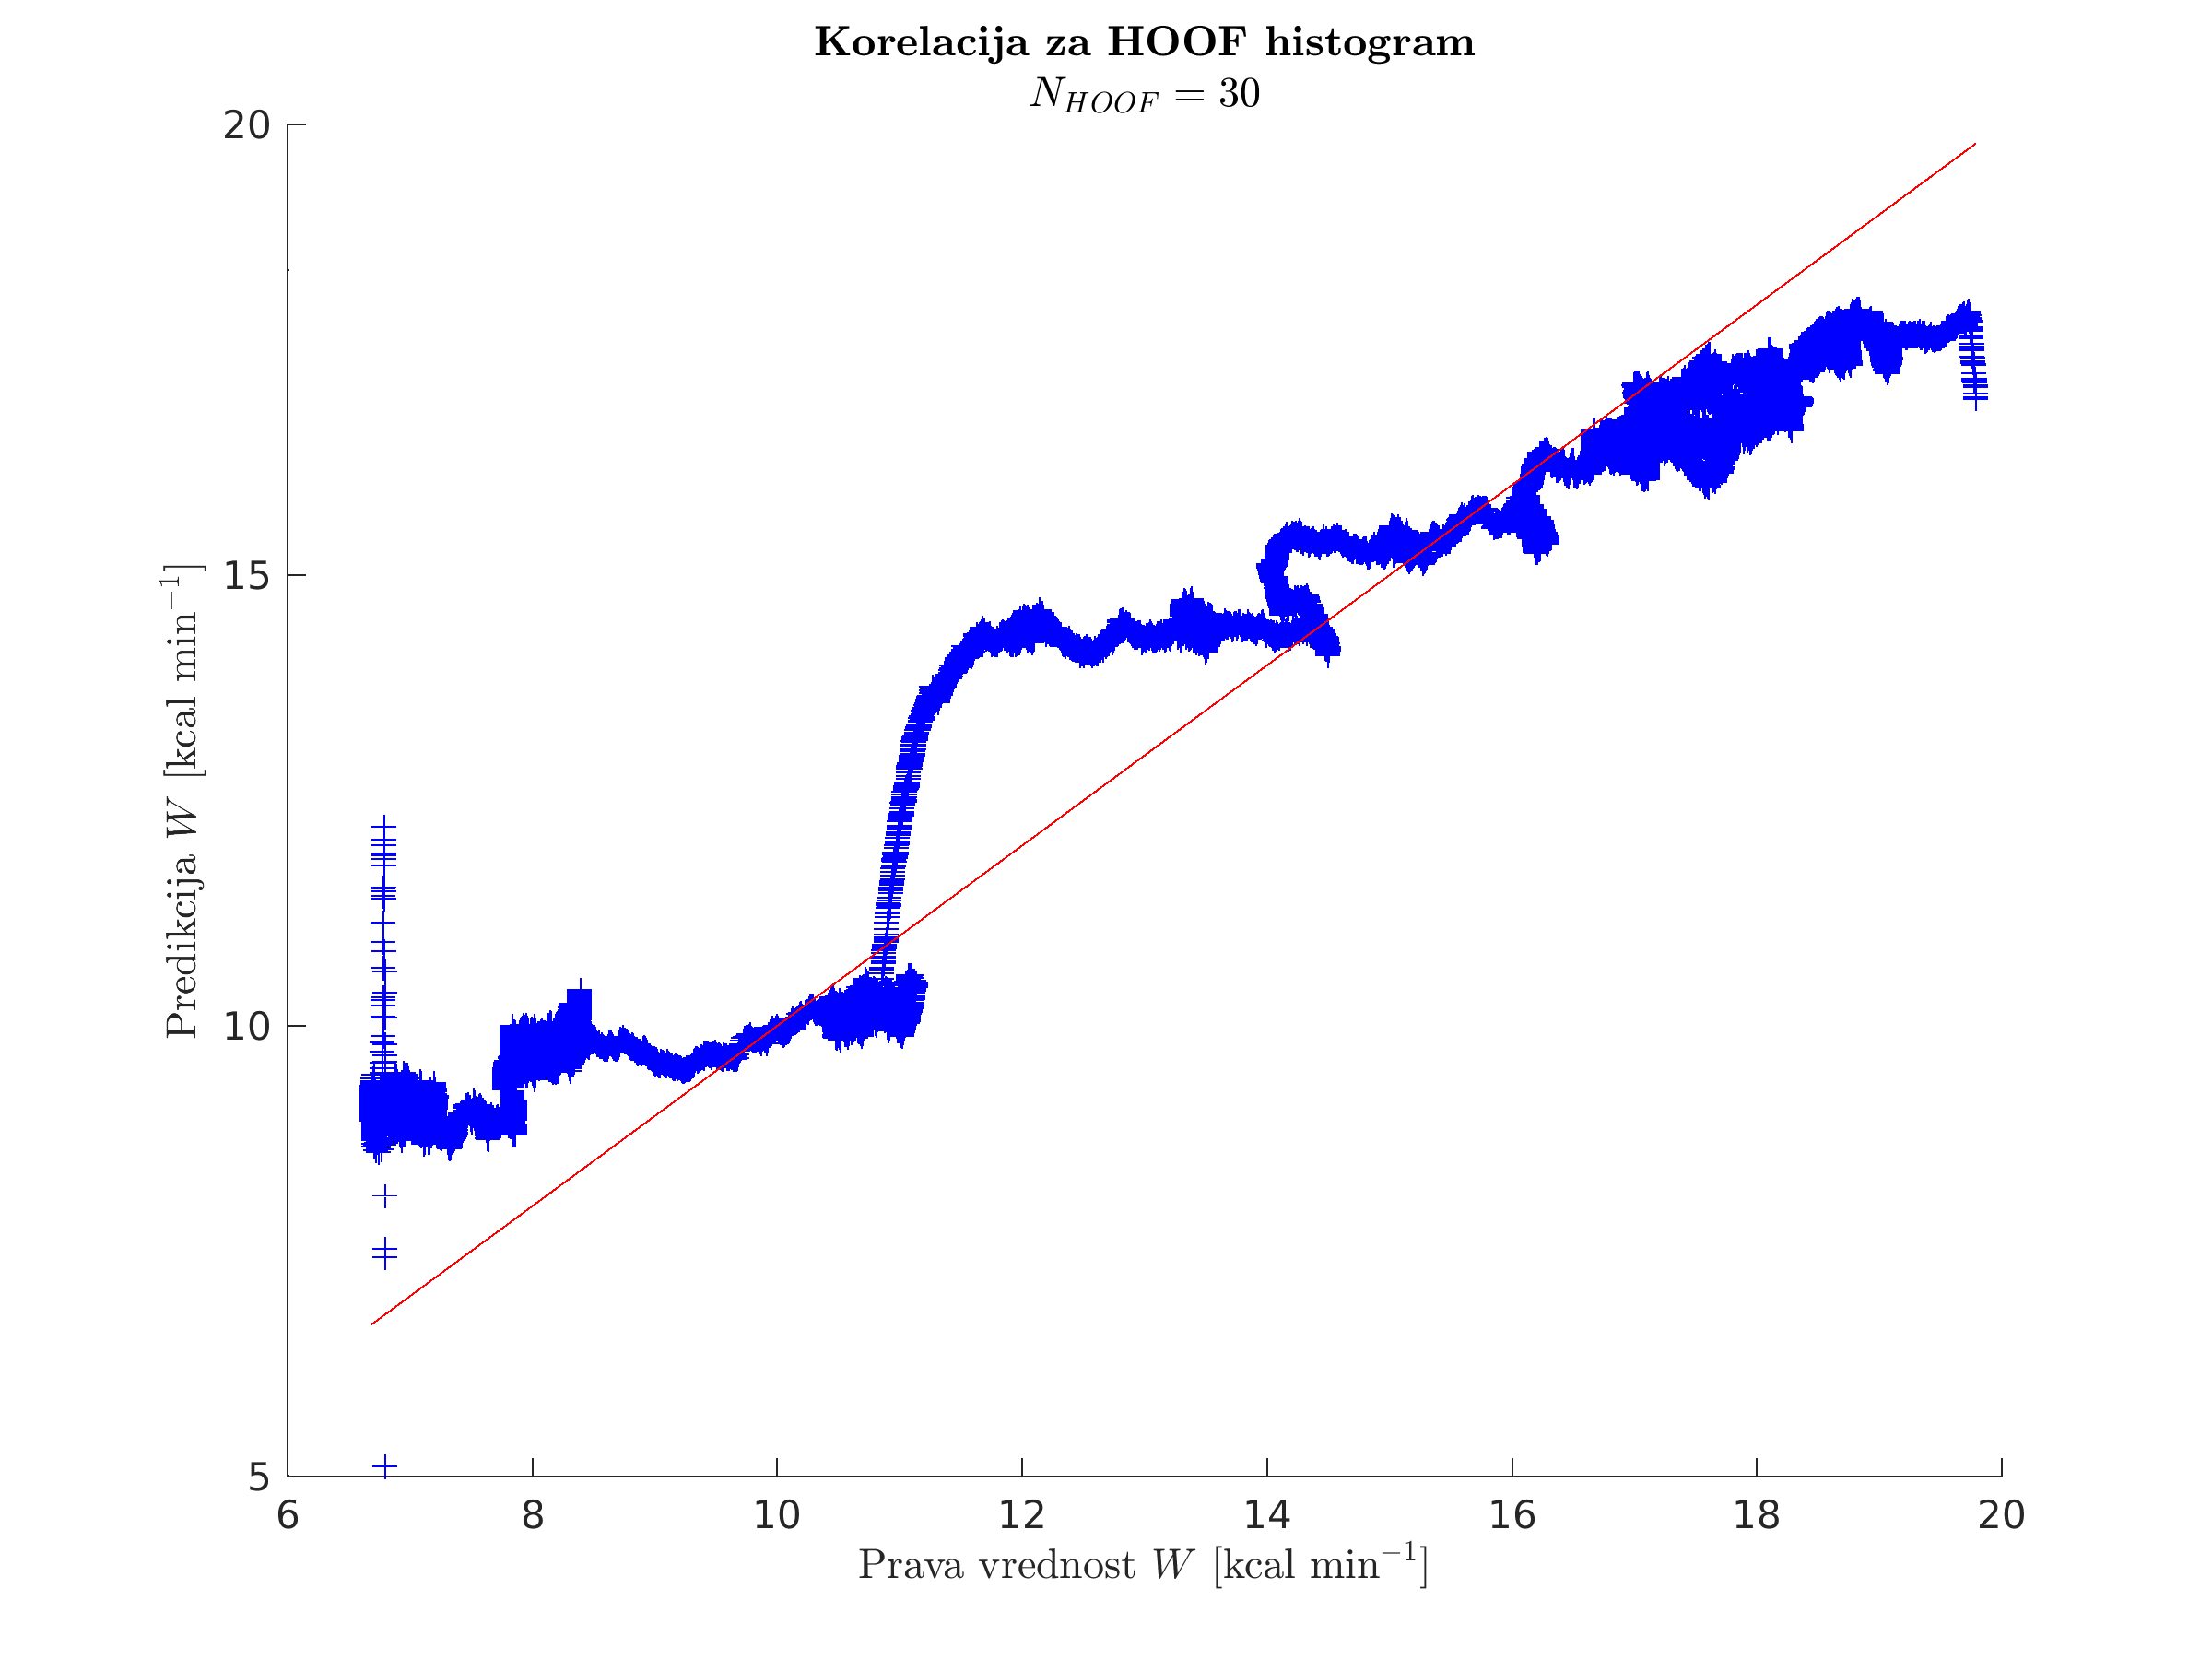
\includegraphics[width=\columnwidth]{./Slike/corr-hoof-30.png}
        \caption{Korelacija $N_{HOOF}=30$.}
        \label{fig:corr-hoof-30}
    \end{subfigure}
    ~
    \begin{subfigure}[t]{0.45\columnwidth}
      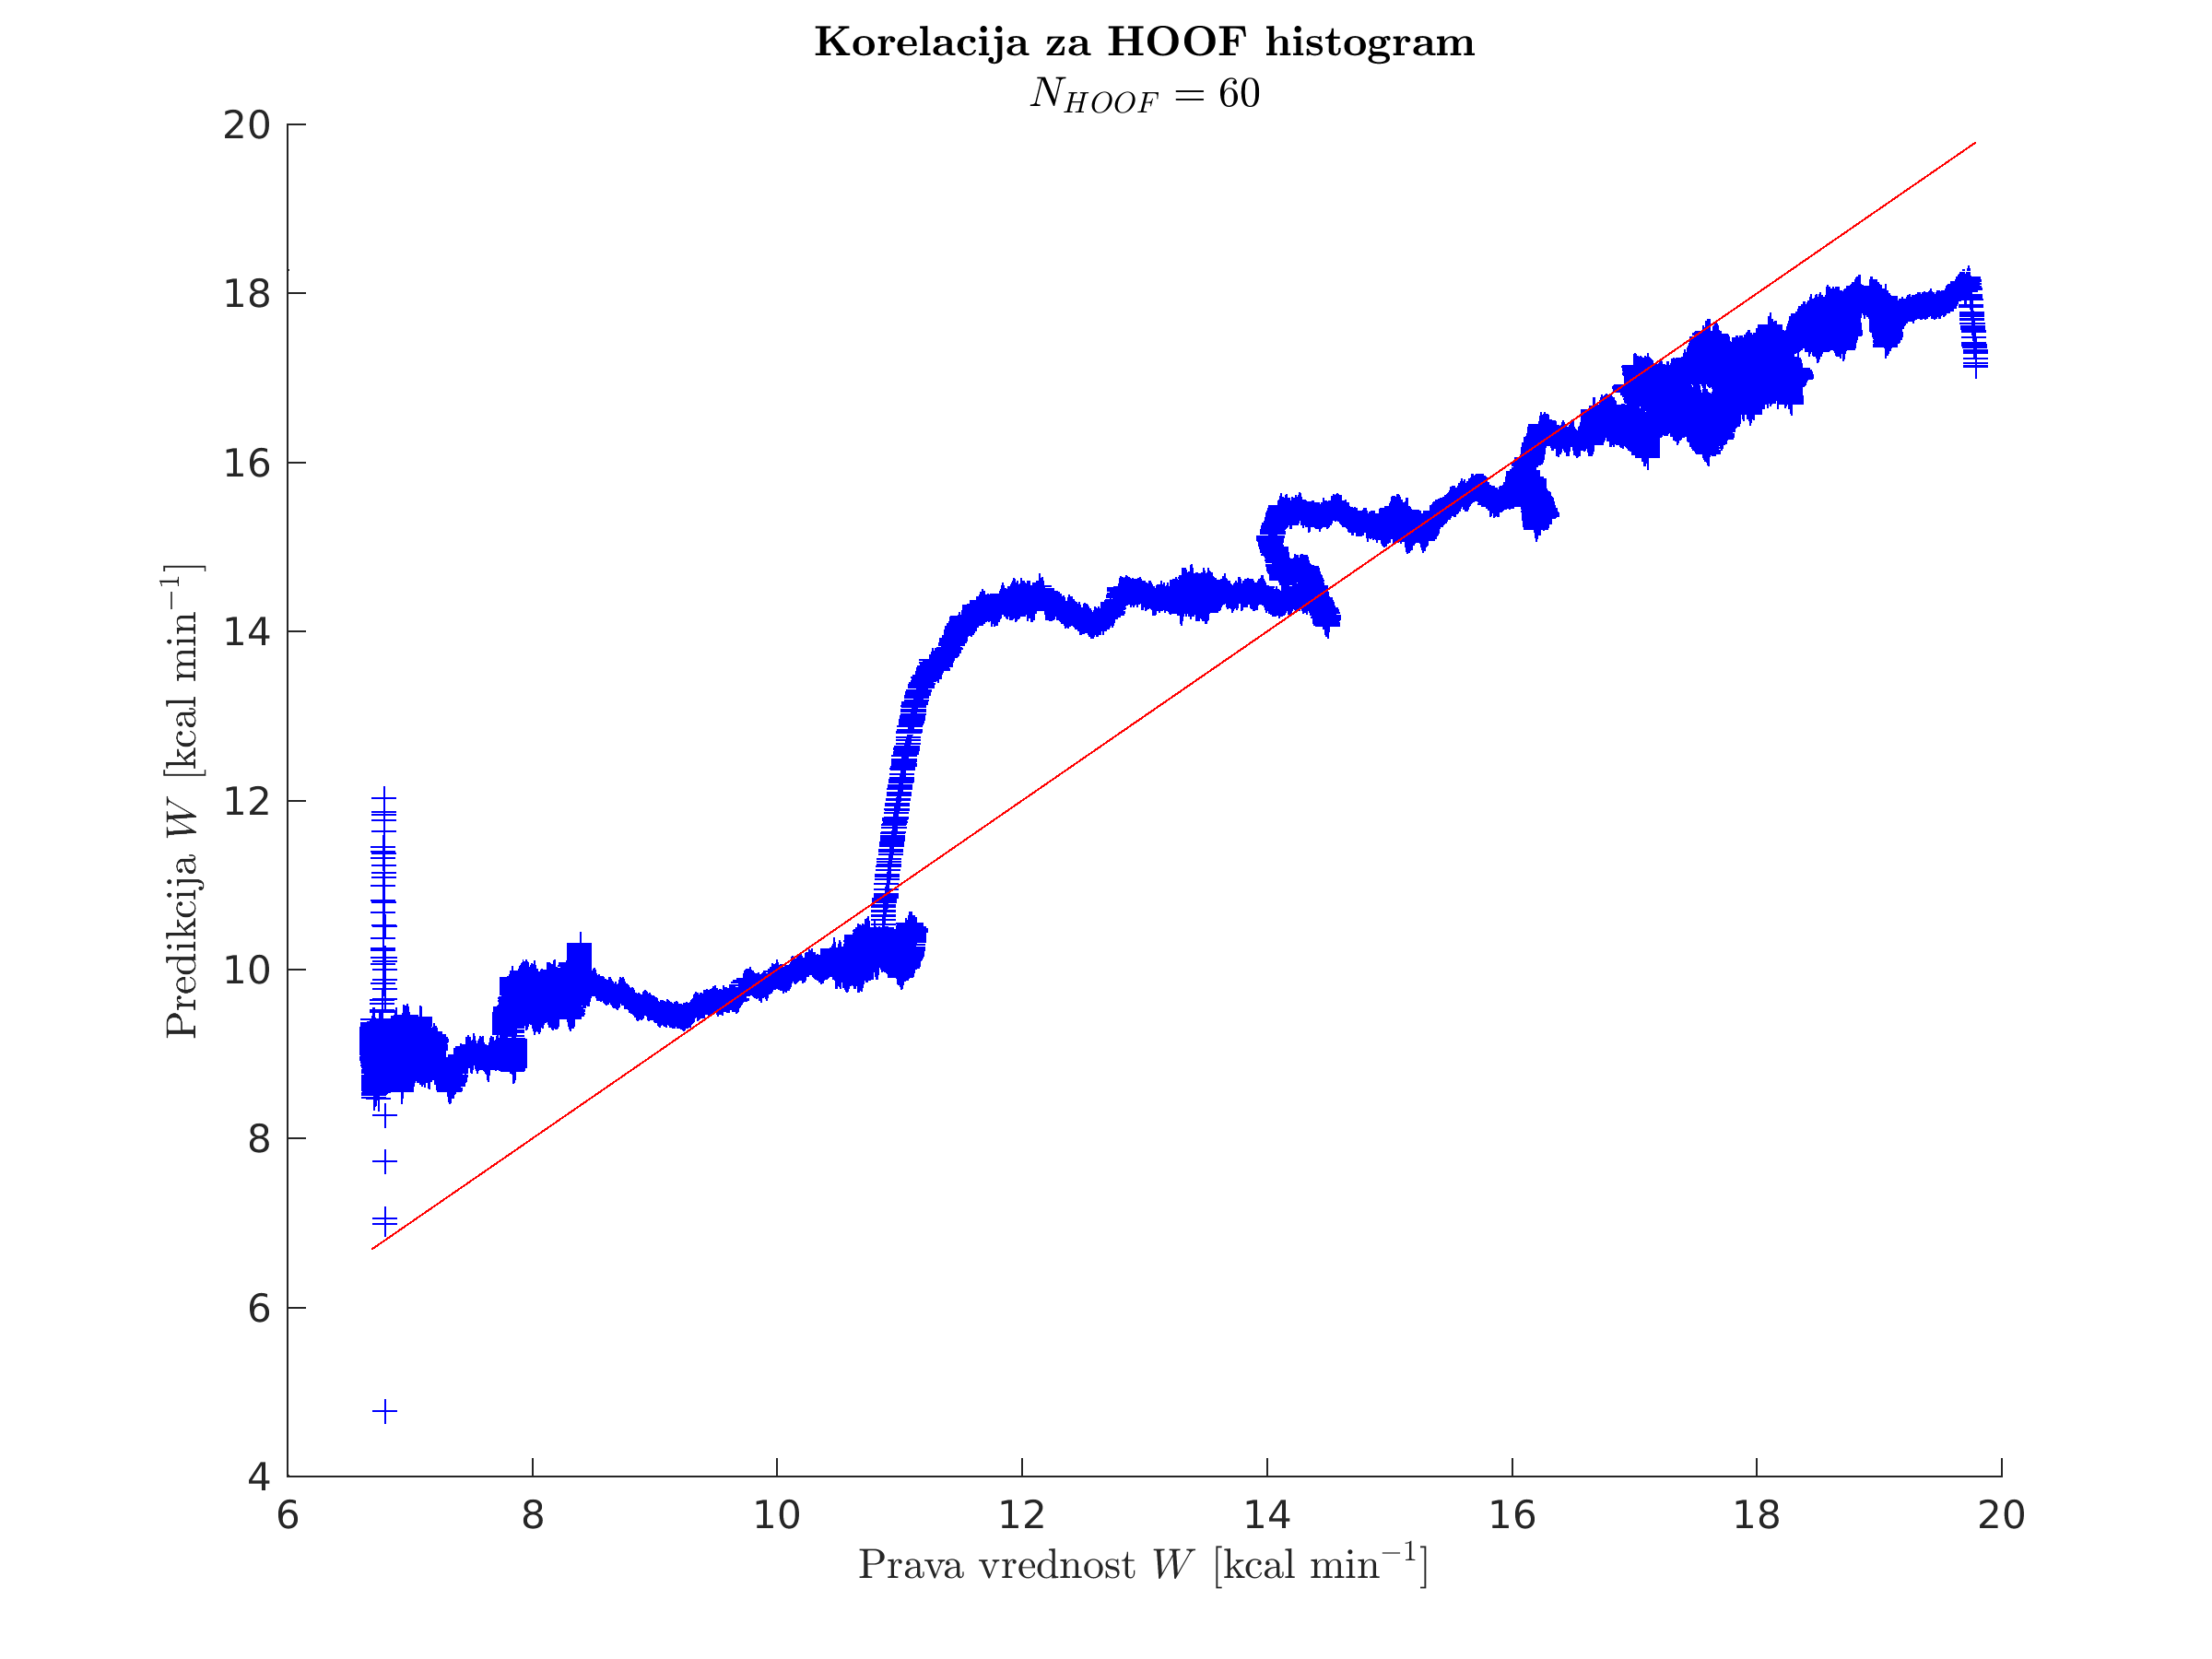
\includegraphics[width=\columnwidth]{./Slike/corr-hoof-60.png}
      \caption{Korelacija $N_{HOOF}=60$.}
      \label{fig:corr-hoof-60}
    \end{subfigure}
    ~
    \begin{subfigure}[b]{0.45\columnwidth}
      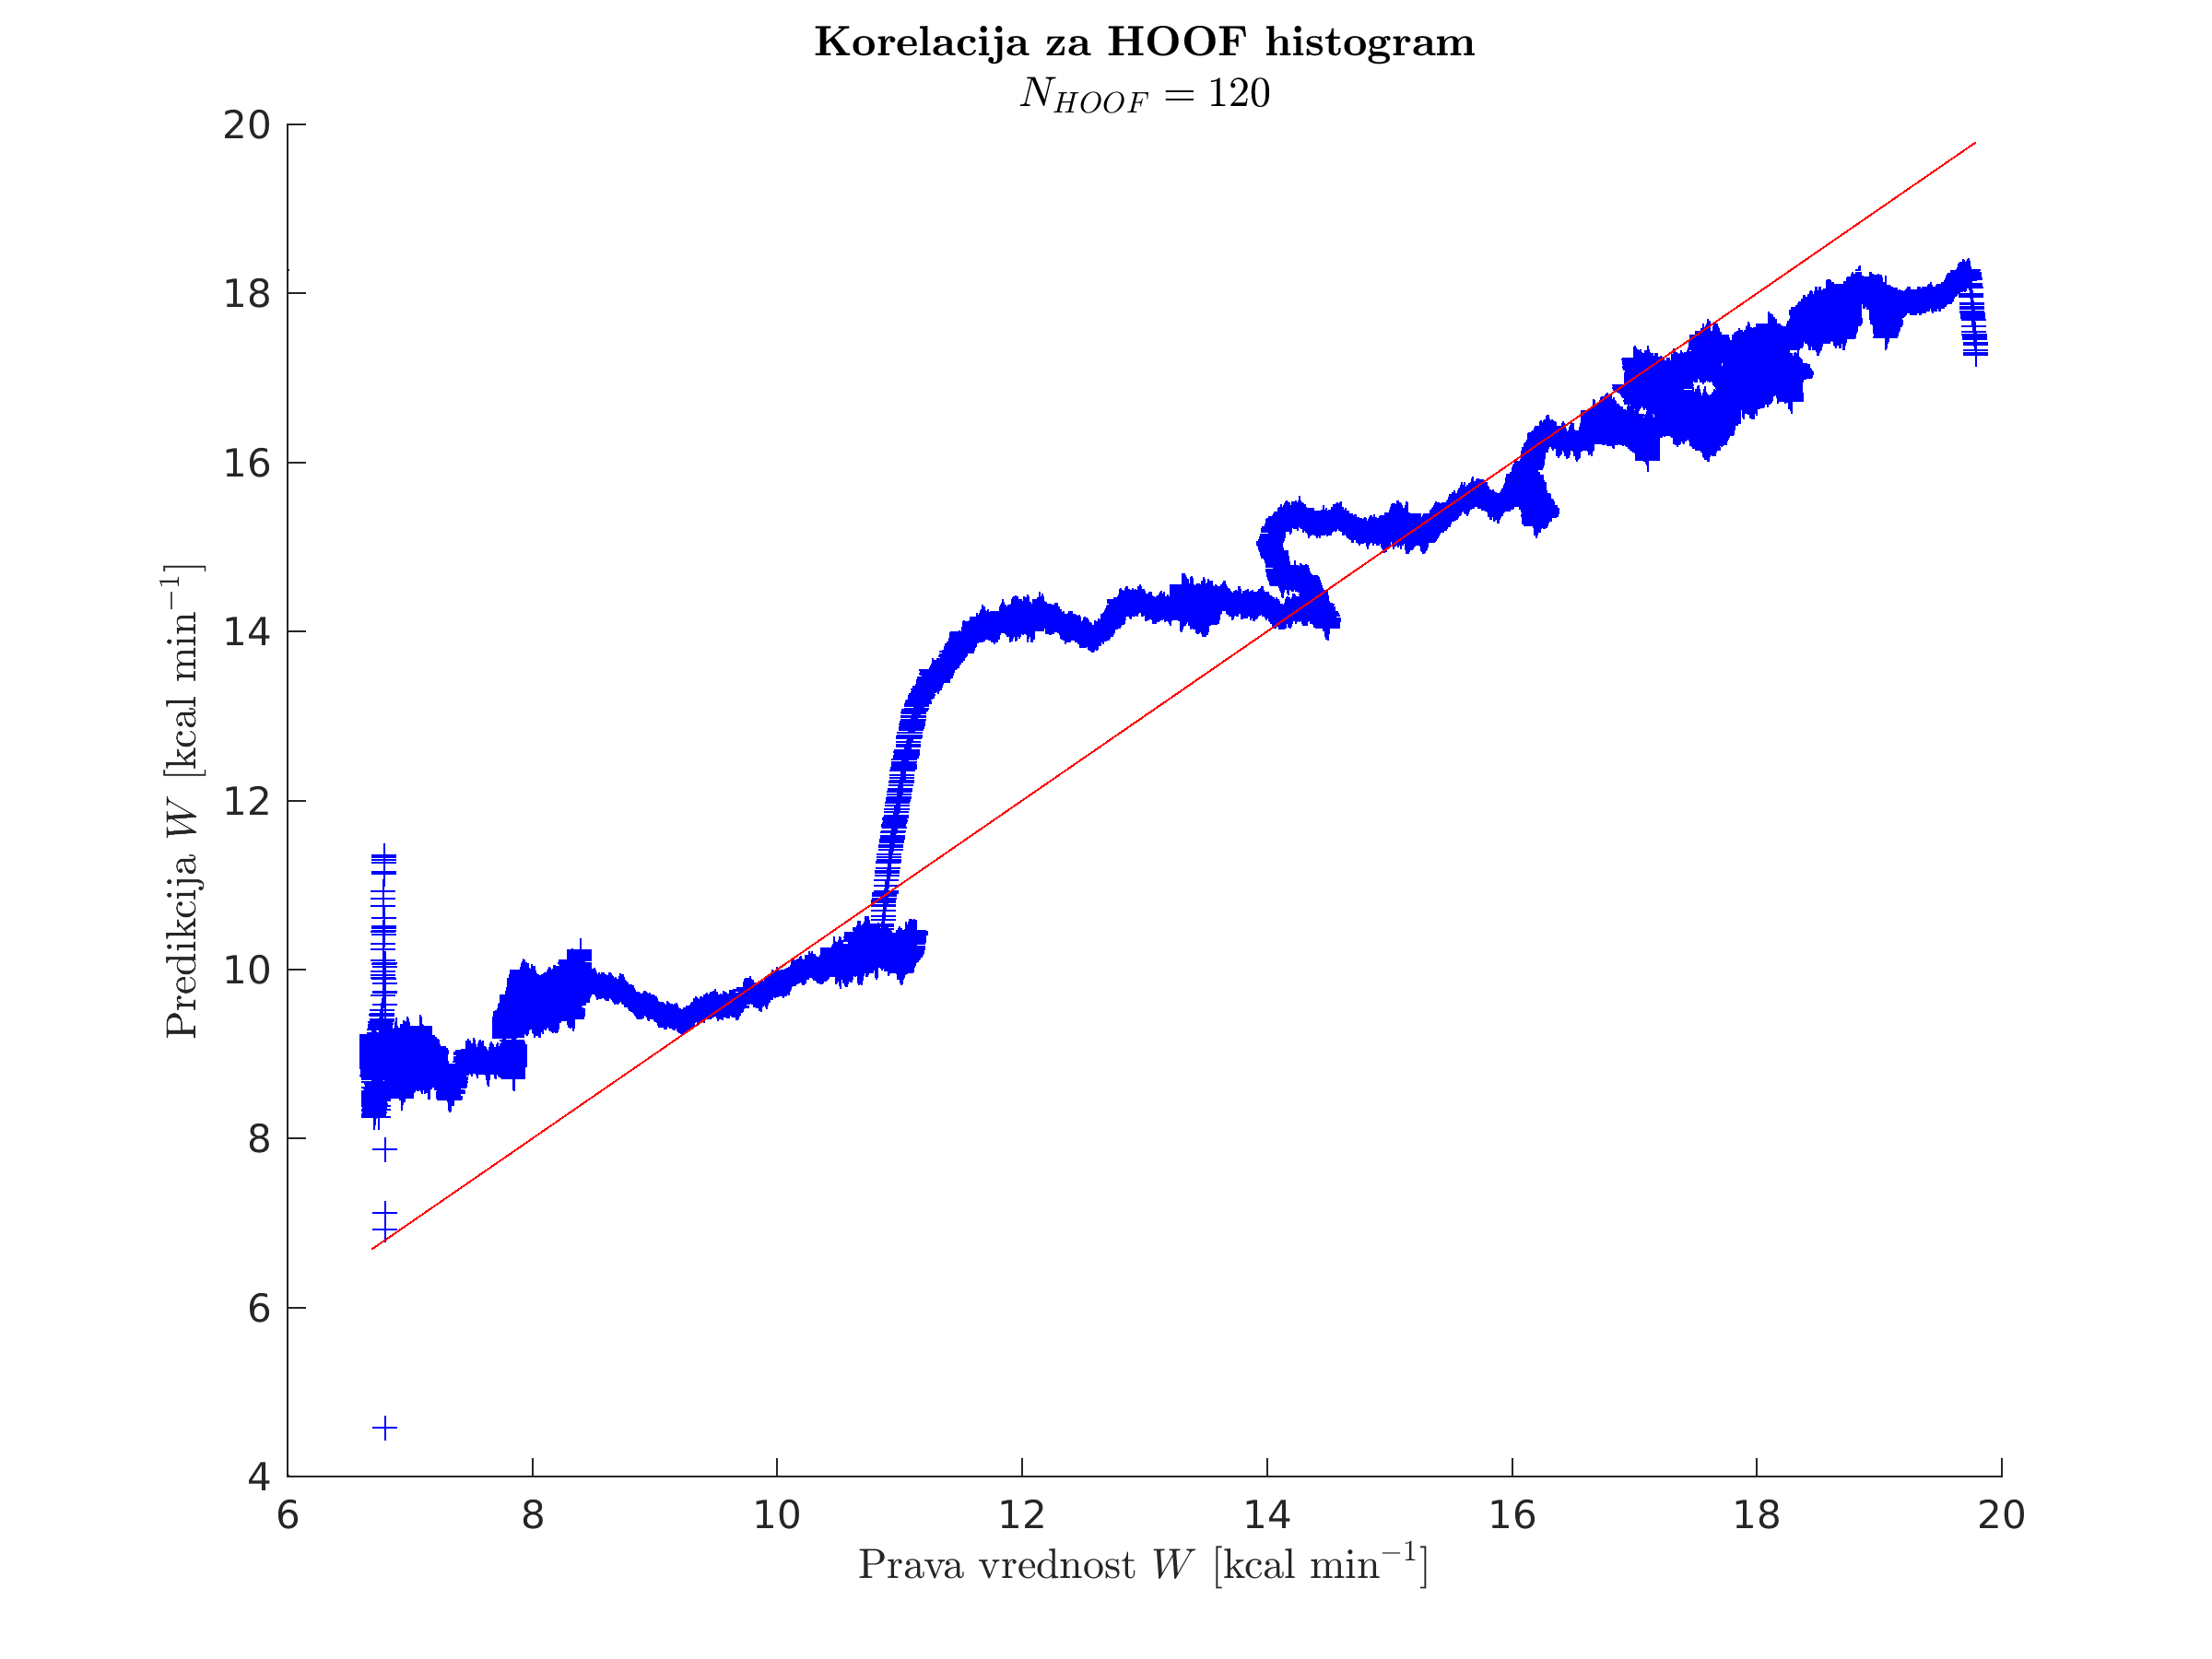
\includegraphics[width=\columnwidth]{./Slike/corr-hoof-120.png}
      \caption{Korelacija $N_{HOOF}=120$.}
      \label{fig:corr-hoof-120}
    \end{subfigure}
    ~
    \begin{subfigure}[b]{0.45\columnwidth}
      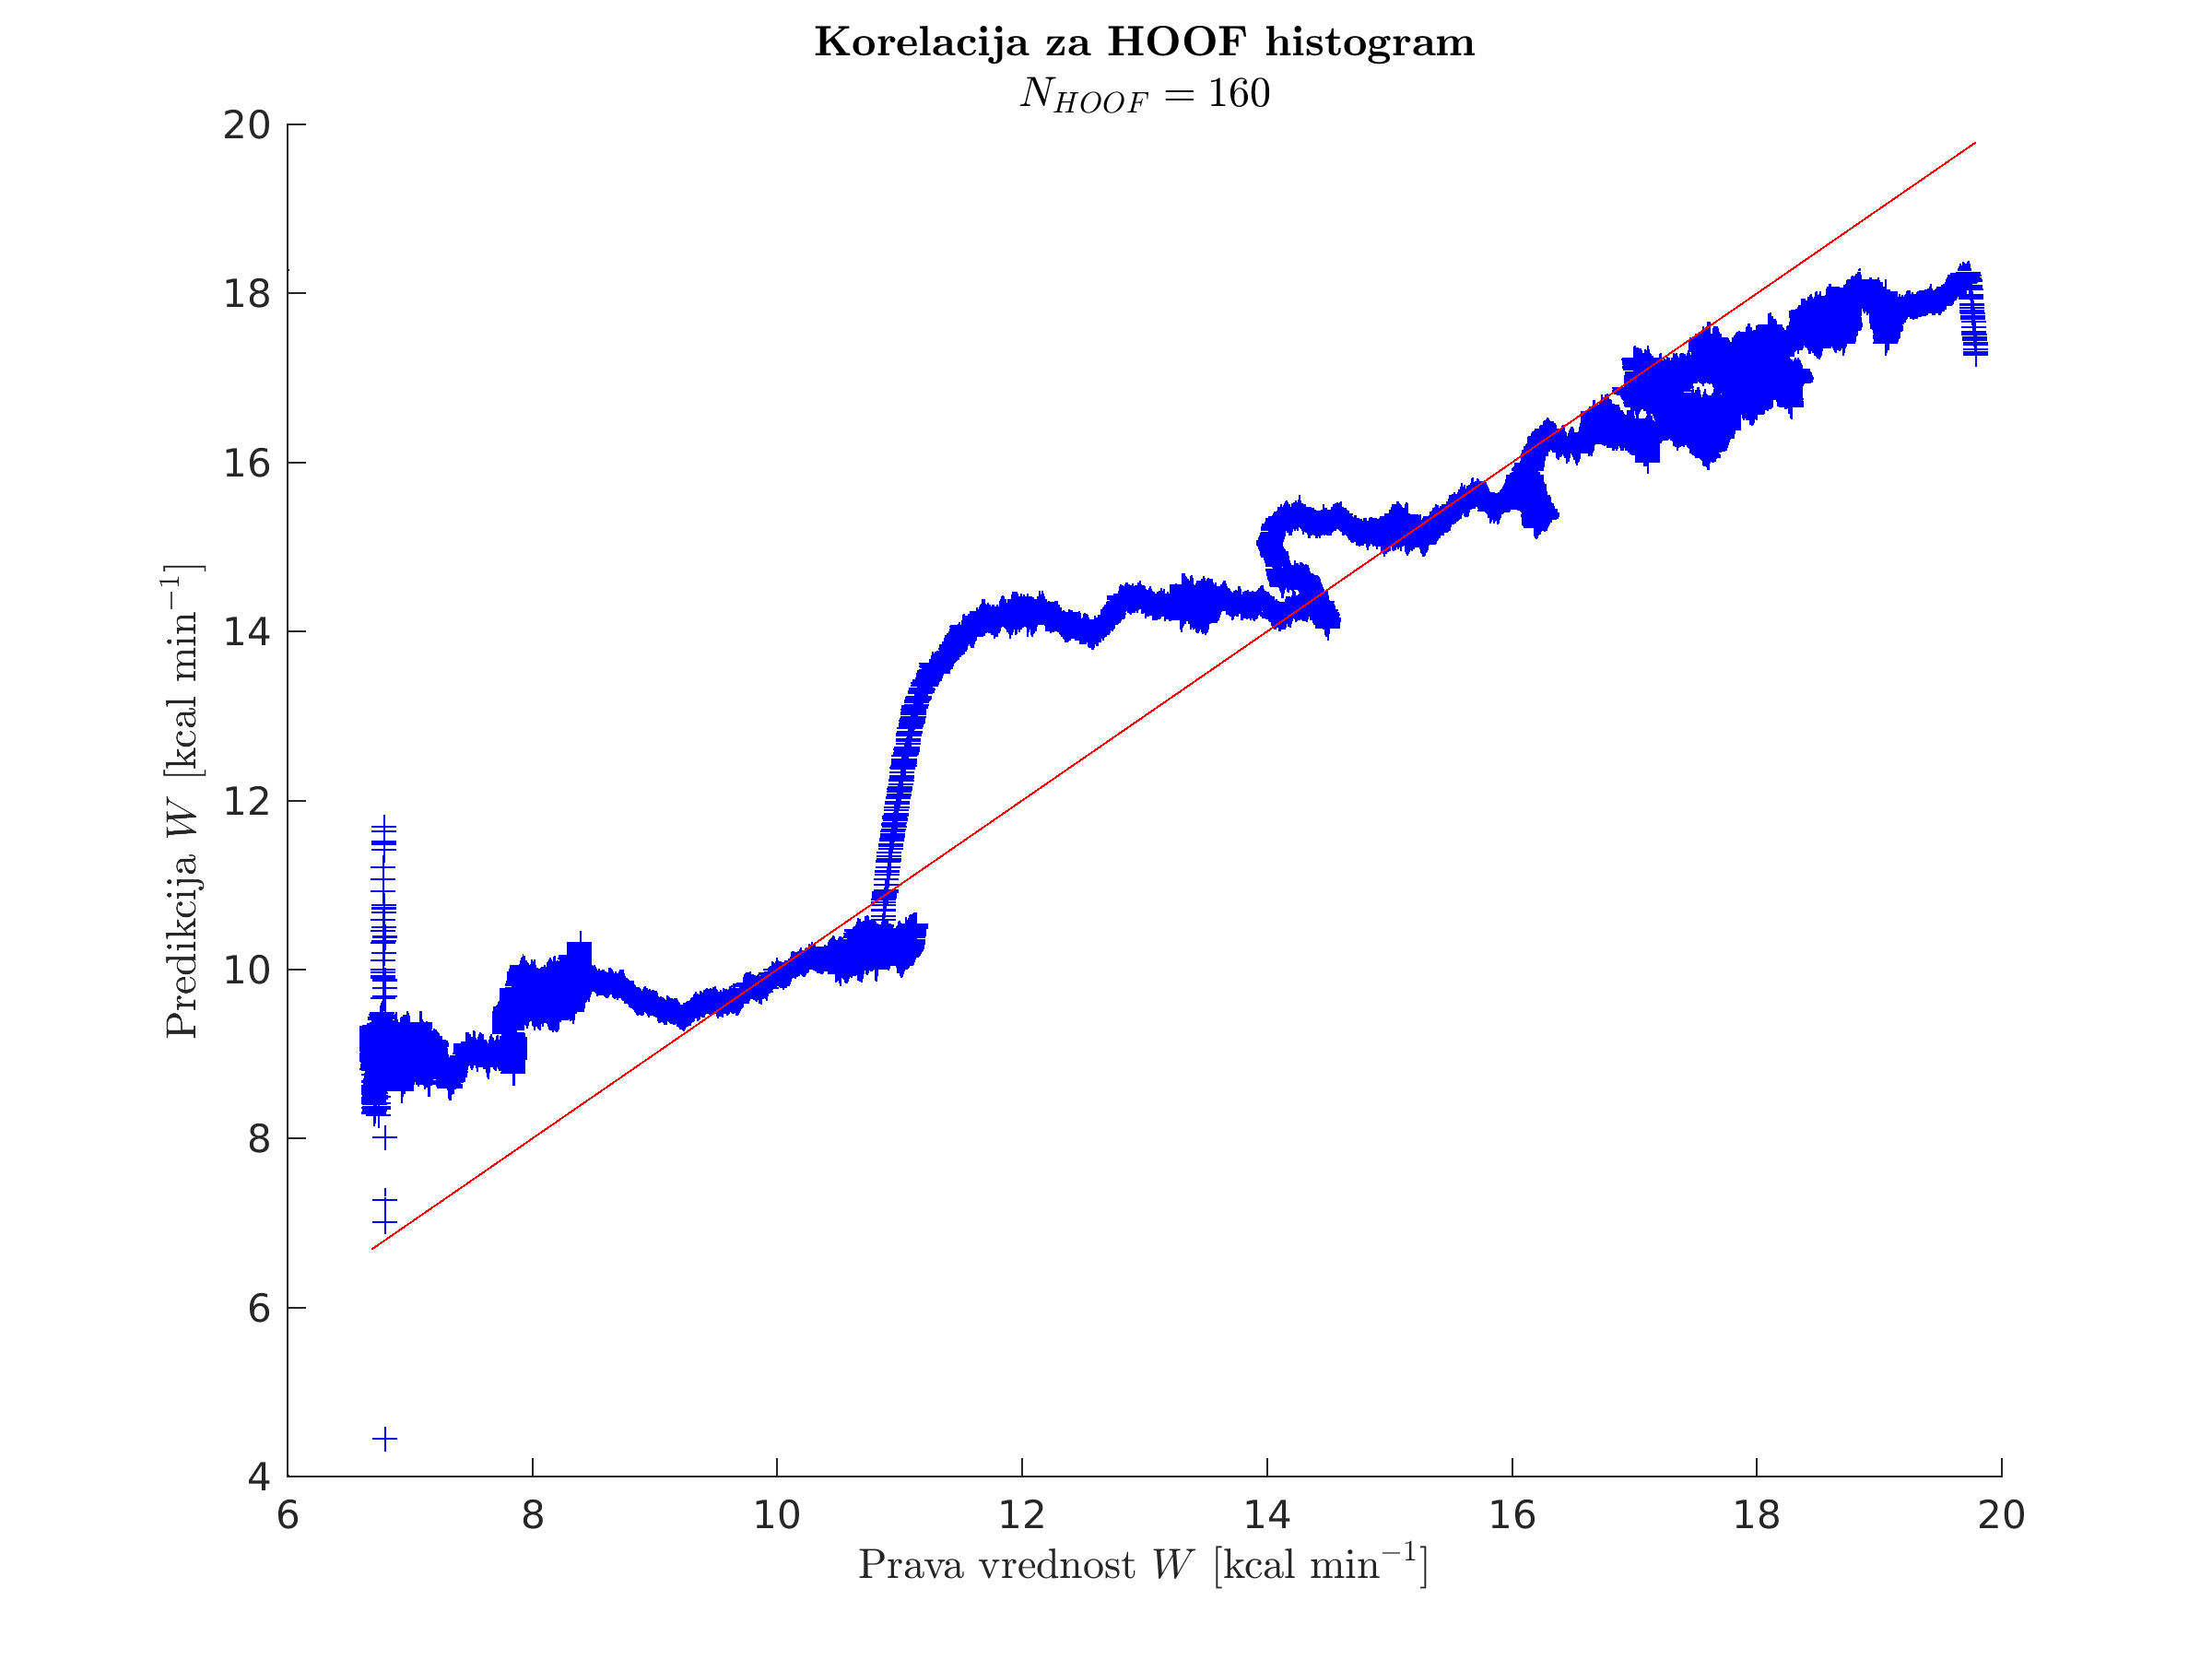
\includegraphics[width=\columnwidth]{./Slike/corr-hoof-160.png}
      \caption{Korelacija $N_{HOOF}=160$.}
      \label{fig:corr-hoof-160}
    \end{subfigure}
    \caption[Grafi korelacij modelov z različnim $N_{HOOF}$]{Grafi korelacij modelov z različnim številom stolpcev $N_{HOOF}$ HOOF deskriptorja. Rezultati so si zelo podobni.}
    \label{fig:corr-hoof}
\end{figure}





\subsubsection{Optimizacija HAFA deskriptorjev}
Parameter $N_{HAFA}$ smo določili na podlagi rezultatov evaluacije v tabeli \ref{tab:nhafa} in grafov korelacije med referenčnimi podatki in predikcijo \ref{fig:corr-hafa}. Za evaluacijo smo uporabili enak eksperimentalni protokol kot za HOOF značilke v poglavju \ref{sec:hoof}, s to razliko, da smo značilke normirali na intervalu $[0, 1]$ in odstranili stolpec z amplitudami $0.5$. S tem smo odstranili šum, ki se je pojavil, ko ni bilo nobenega gibanja. Amplitudo šuma smo določili, kot maksimalno vrednost amplitude, ki še ni predstavljala gibanja. Optimalni parametri evaluacijske metode so predstavljeni v tabeli \ref{tab:nhafa-param}.


\begin{table}[htb]
	\centering
    \begin{tabular}{S[table-format=2.0] S[table-format=2.3] S[table-format=1.3]  S[table-format=1.3] S[table-format=1.3]}
    \toprule
    \thead{$\mathbf{N_{HAFA}}$} & \thead{$\mathbf{C}$} & \thead{$\mathbf{\gamma}$} & \thead{$\mathbf{\epsilon}$} & \thead{MSE} \\ 
    \midrule
    30 & 8 & 5.657 & 0.616 & 4.329 \\
    60 & 8 & 5.657 & 0.616 & 4.327 \\
    120 & 8 & 5.657 & 0.616 & 4.327 \\
    160 & 8 & 5.657 & 0.616 & 4.327 \\
    \bottomrule
    \end{tabular}
    \caption[Optimalni parameteri RBF jedra modelov za določitev $N_{HAFA}$]{Optimalni parametri RBF jedra za modele z različnim številom stolpcev $N_{HAFA}$ v HAFA deskriptorju.}
    \label{tab:nhafa-param}
\end{table}

V tabeli \ref{tab:nhafa} lahko vidimo, da so rezultati praktično enaki. Za našo metodo smo izbrali $N_{HAFA}=60$, kar v grobem predstavlja $60$ različnih hitrosti z maksimalno amplitudo \SI{60}{px.f^{-1}}.

\begin{table}[htb]
	\centering
    \begin{tabular}{S[table-format=2.0] S[table-format=1.3] S[table-format=1.3] S[table-format=1.3] S[table-format=2.2]}
    \toprule
    \thead{$\mathbf{N_{HAFA}}$} & \thead{$\mathbf{r}$} & \thead{RAE} & \thead{RRSE} & \thead{nSV [\%]}\\
    \midrule%nSV
    30 & 0.984 & 0.213 & 0.231 & 62.08 \\%17879/28799
    \boldentry{2.0}{60} & \boldentry{1.3}{0.984} & \boldentry{1.3}{0.211} & \boldentry{1.3}{0.228} & \boldentry{2.2}{62.60} \\%18028
    120 & 0.984 & 0.211 & 0.228 & 62.63 \\%18037
    160 & 0.984 & 0.211 & 0.228 & 62.63 \\%18037
    \bottomrule
    \end{tabular}
    \caption[Rezultati evaluacije modelov z različnim $N_{HAFA}$]{Rezultati evaluacije modelov z različnim številom stolpcev $N_{HAFA}$ HAFA deskriptorja. Optimalni rezultati so odebeljeni.}
    \label{tab:nhafa}
\end{table}

\begin{figure}[htb]
	\centering
    \begin{subfigure}[t]{0.45\columnwidth}
    	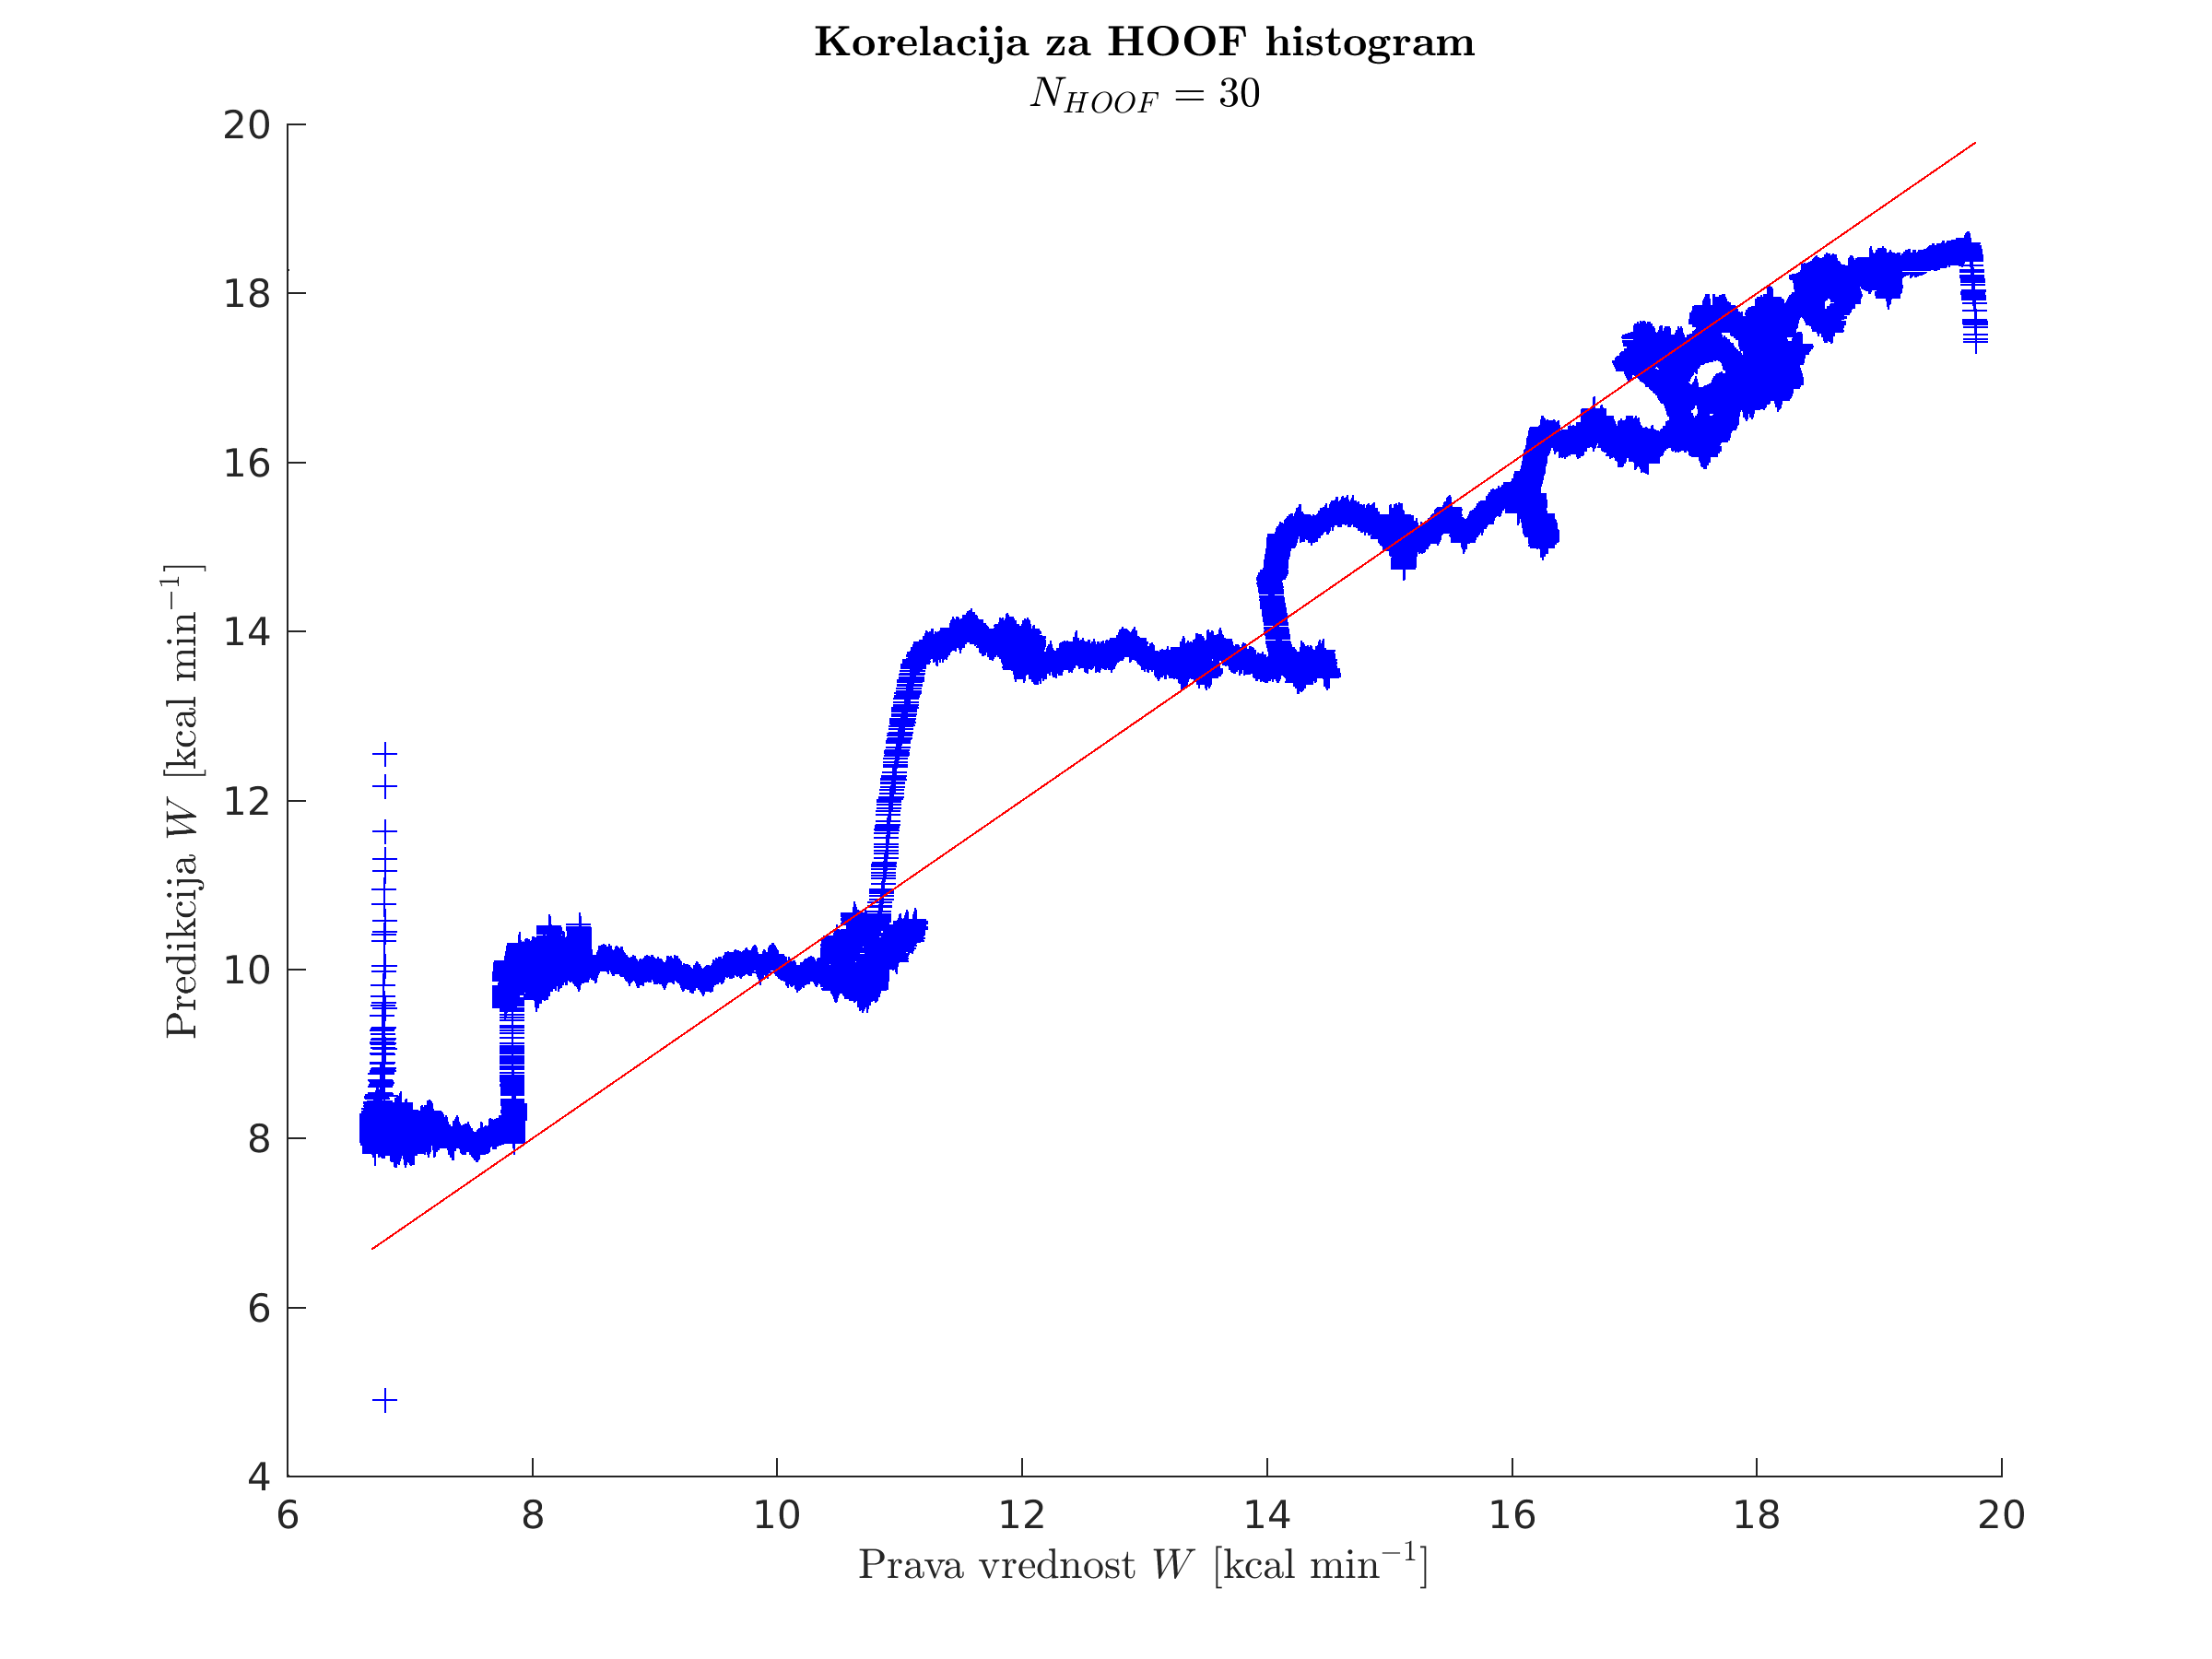
\includegraphics[width=\columnwidth]{./Slike/corr-hafa-30.png}
        \caption{Korelacija $N_{HAFA}=30$.}
        \label{fig:corr-hafa-30}
    \end{subfigure}
    ~
    \begin{subfigure}[t]{0.45\columnwidth}
      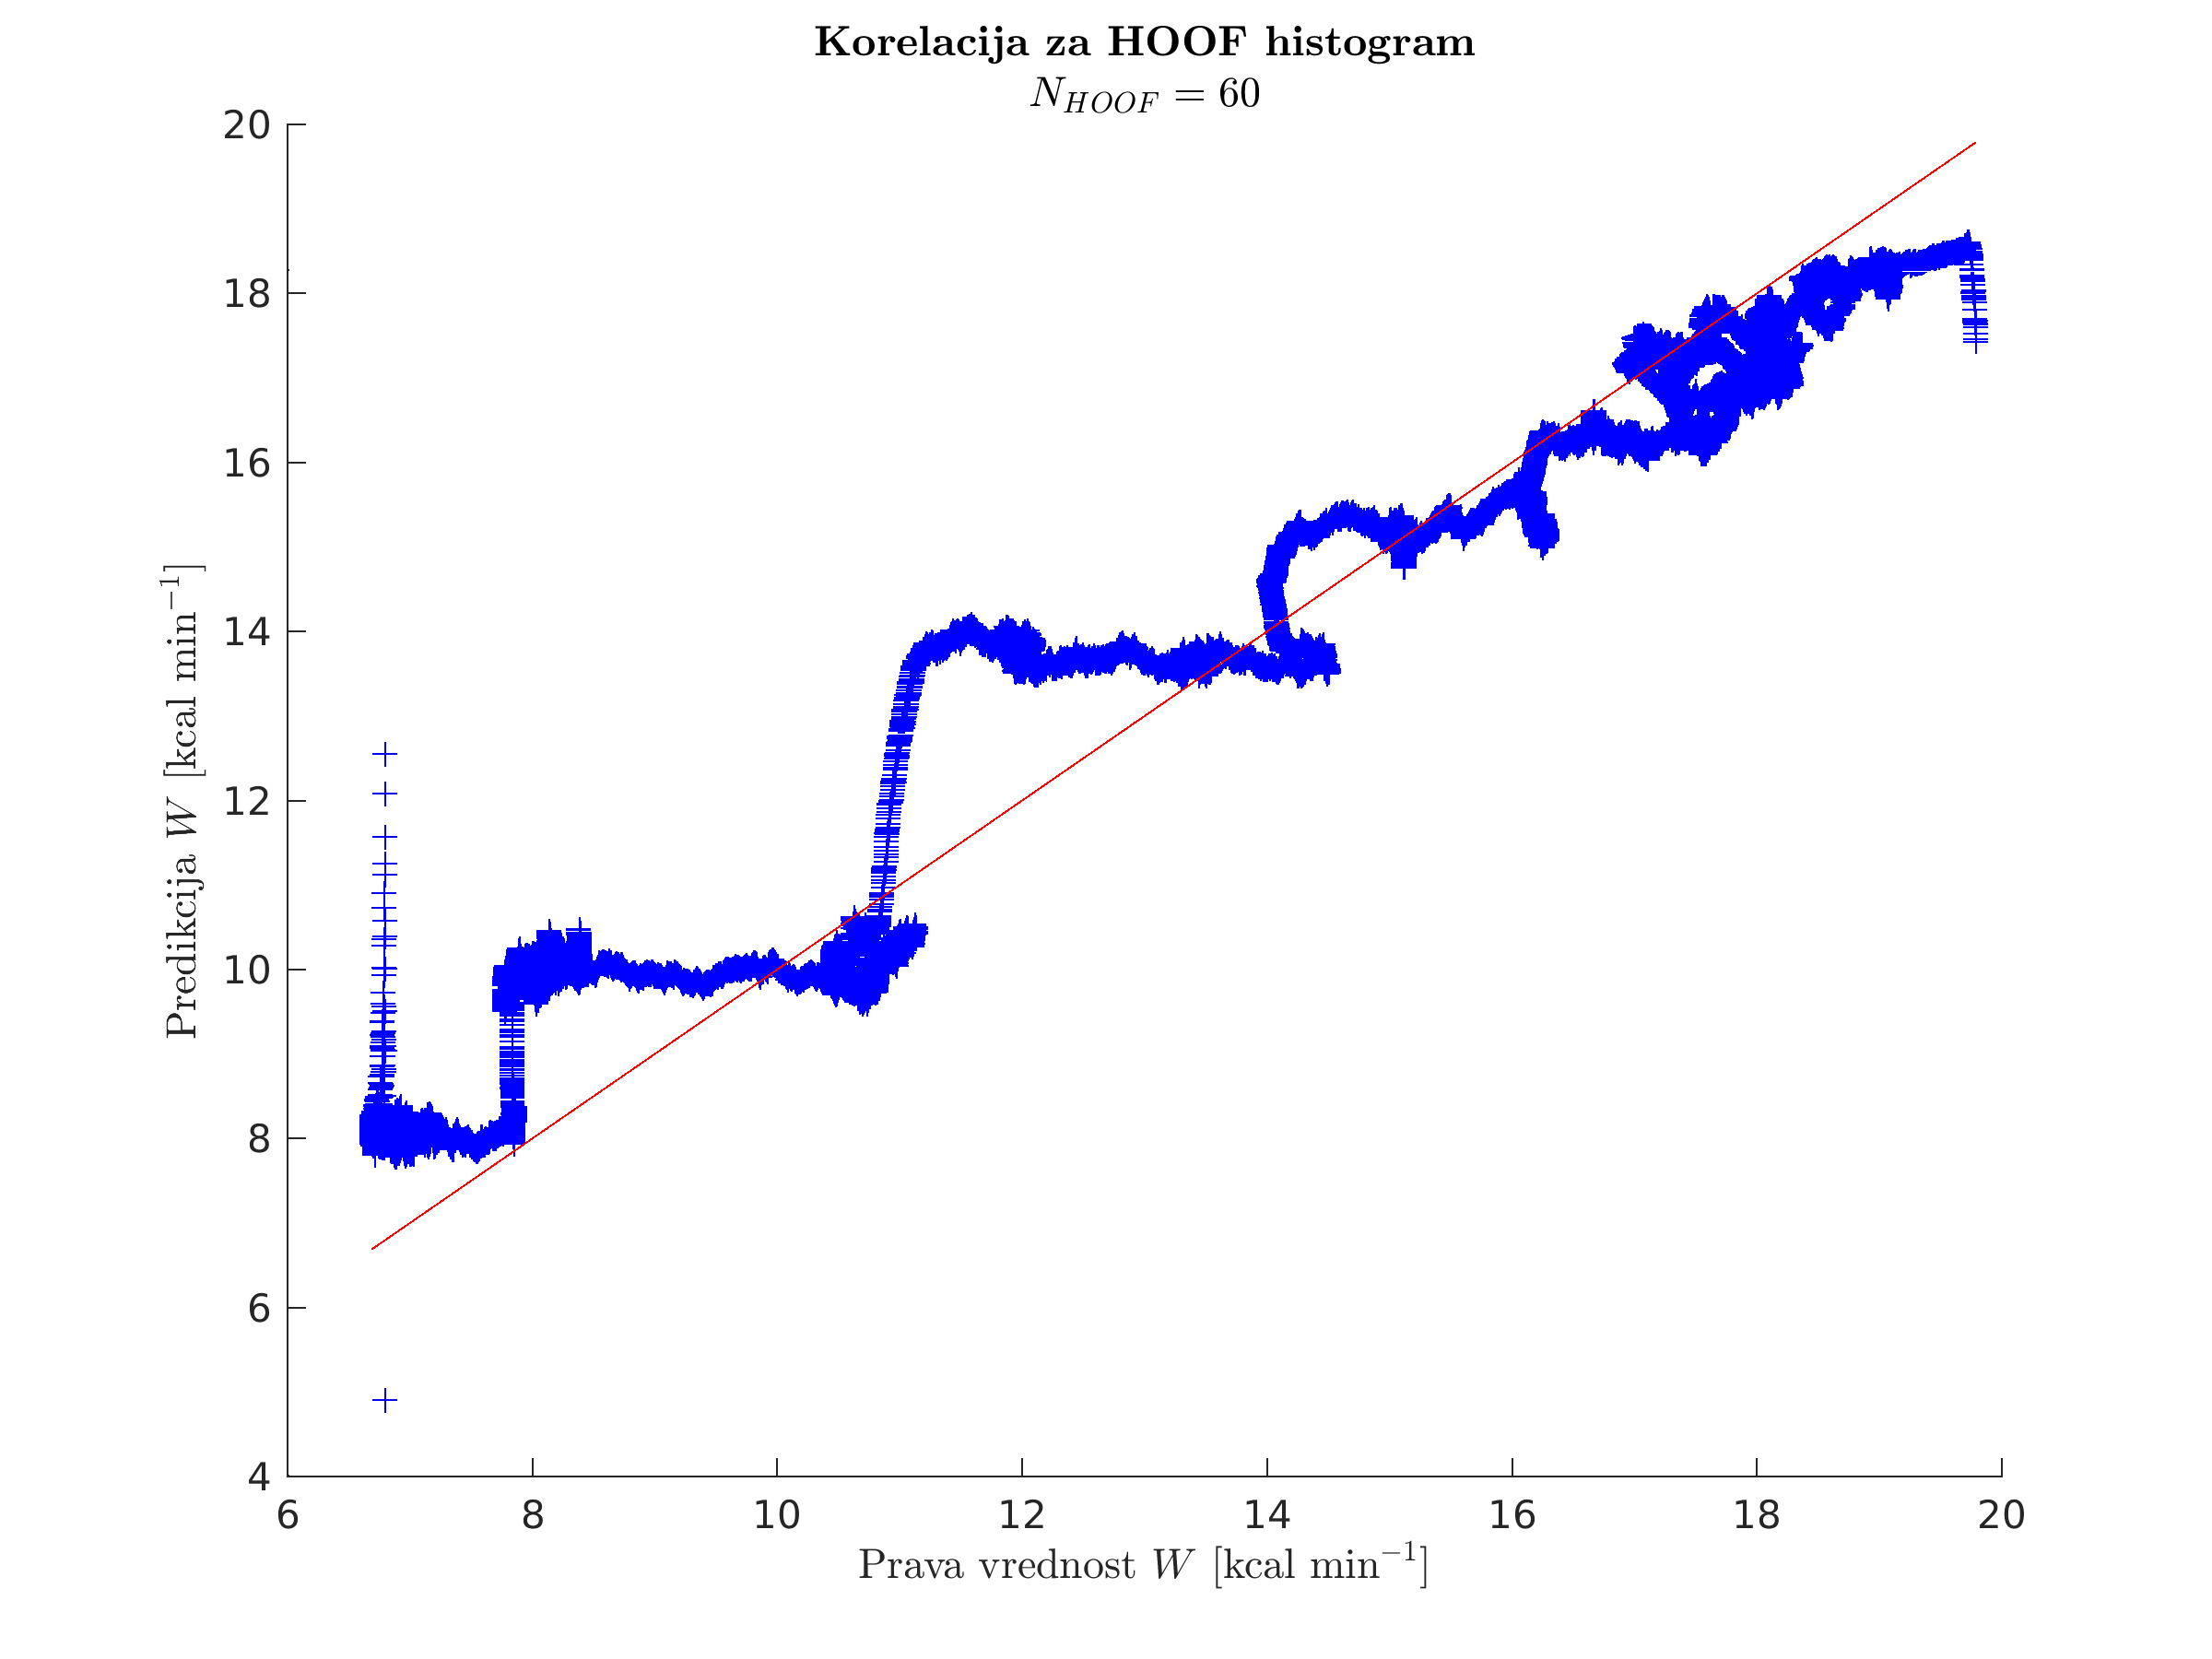
\includegraphics[width=\columnwidth]{./Slike/corr-hafa-60.png}
      \caption{Korelacija $N_{HAFA}=60$.}
      \label{fig:corr-hafa-60}
    \end{subfigure}
    ~
    \begin{subfigure}[b]{0.45\columnwidth}
      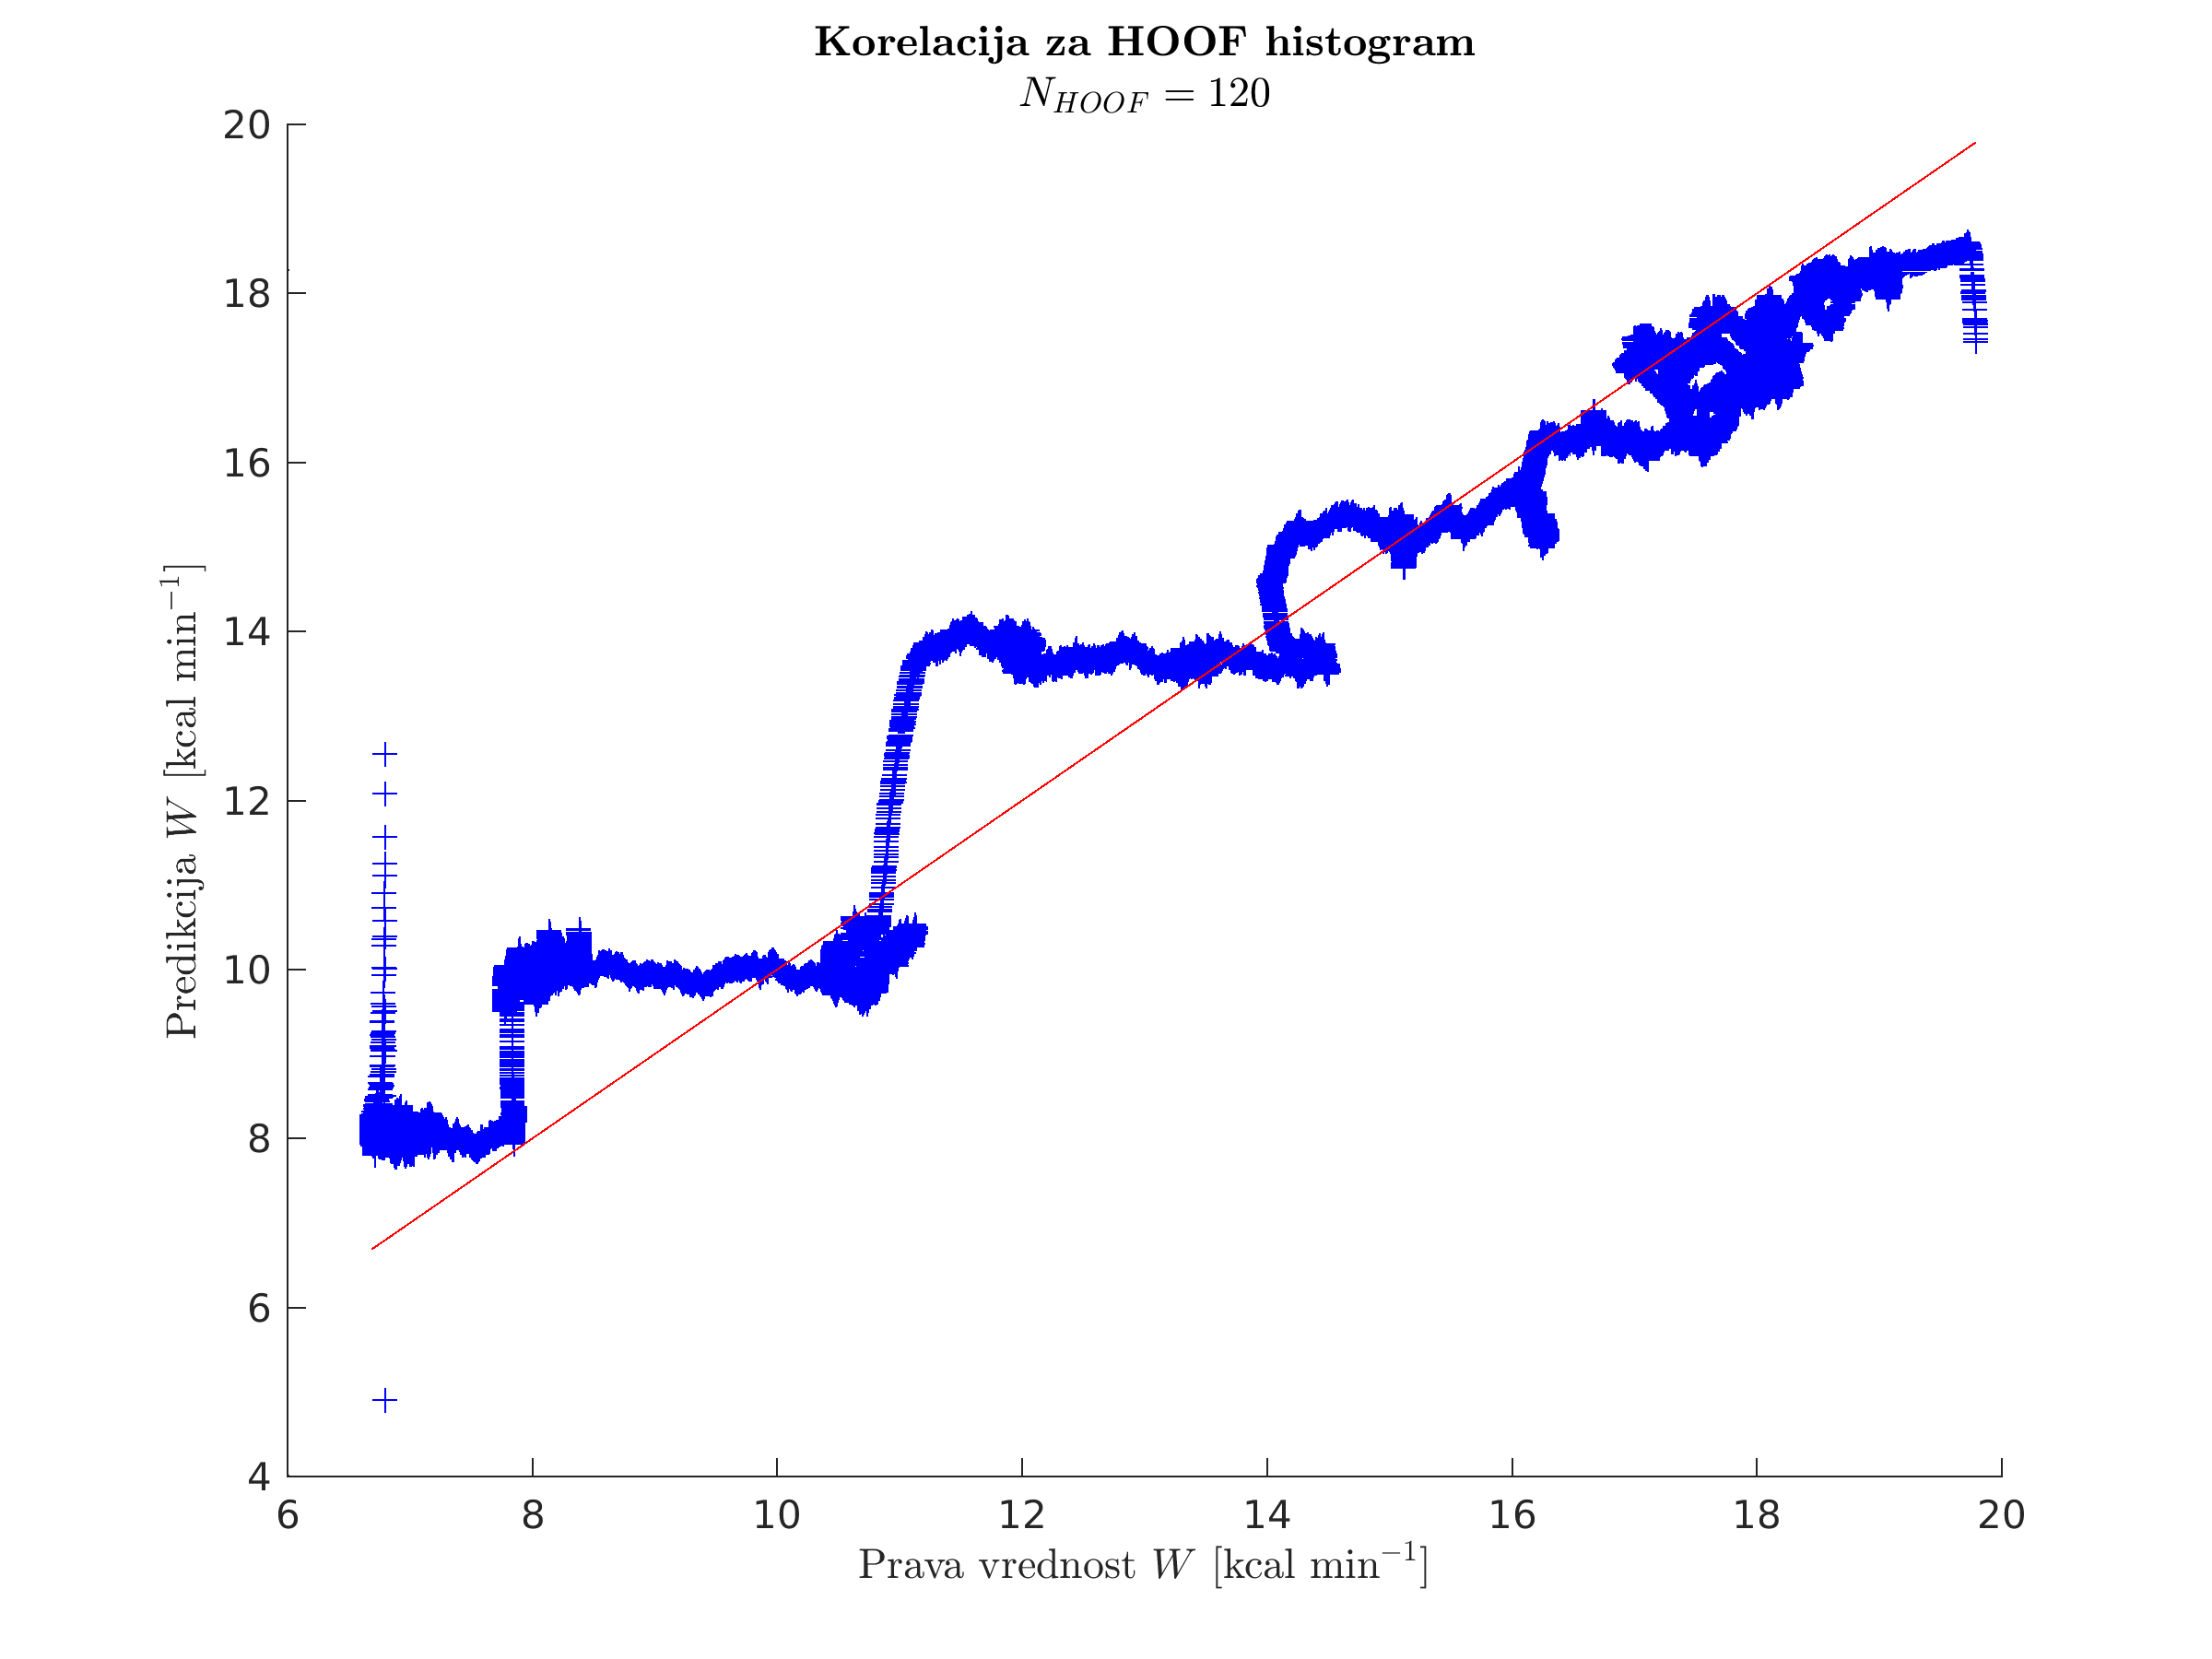
\includegraphics[width=\columnwidth]{./Slike/corr-hafa-120.png}
      \caption{Korelacija $N_{HAFA}=120$.}
      \label{fig:corr-hafa-120}
    \end{subfigure}
    ~
    \begin{subfigure}[b]{0.45\columnwidth}
      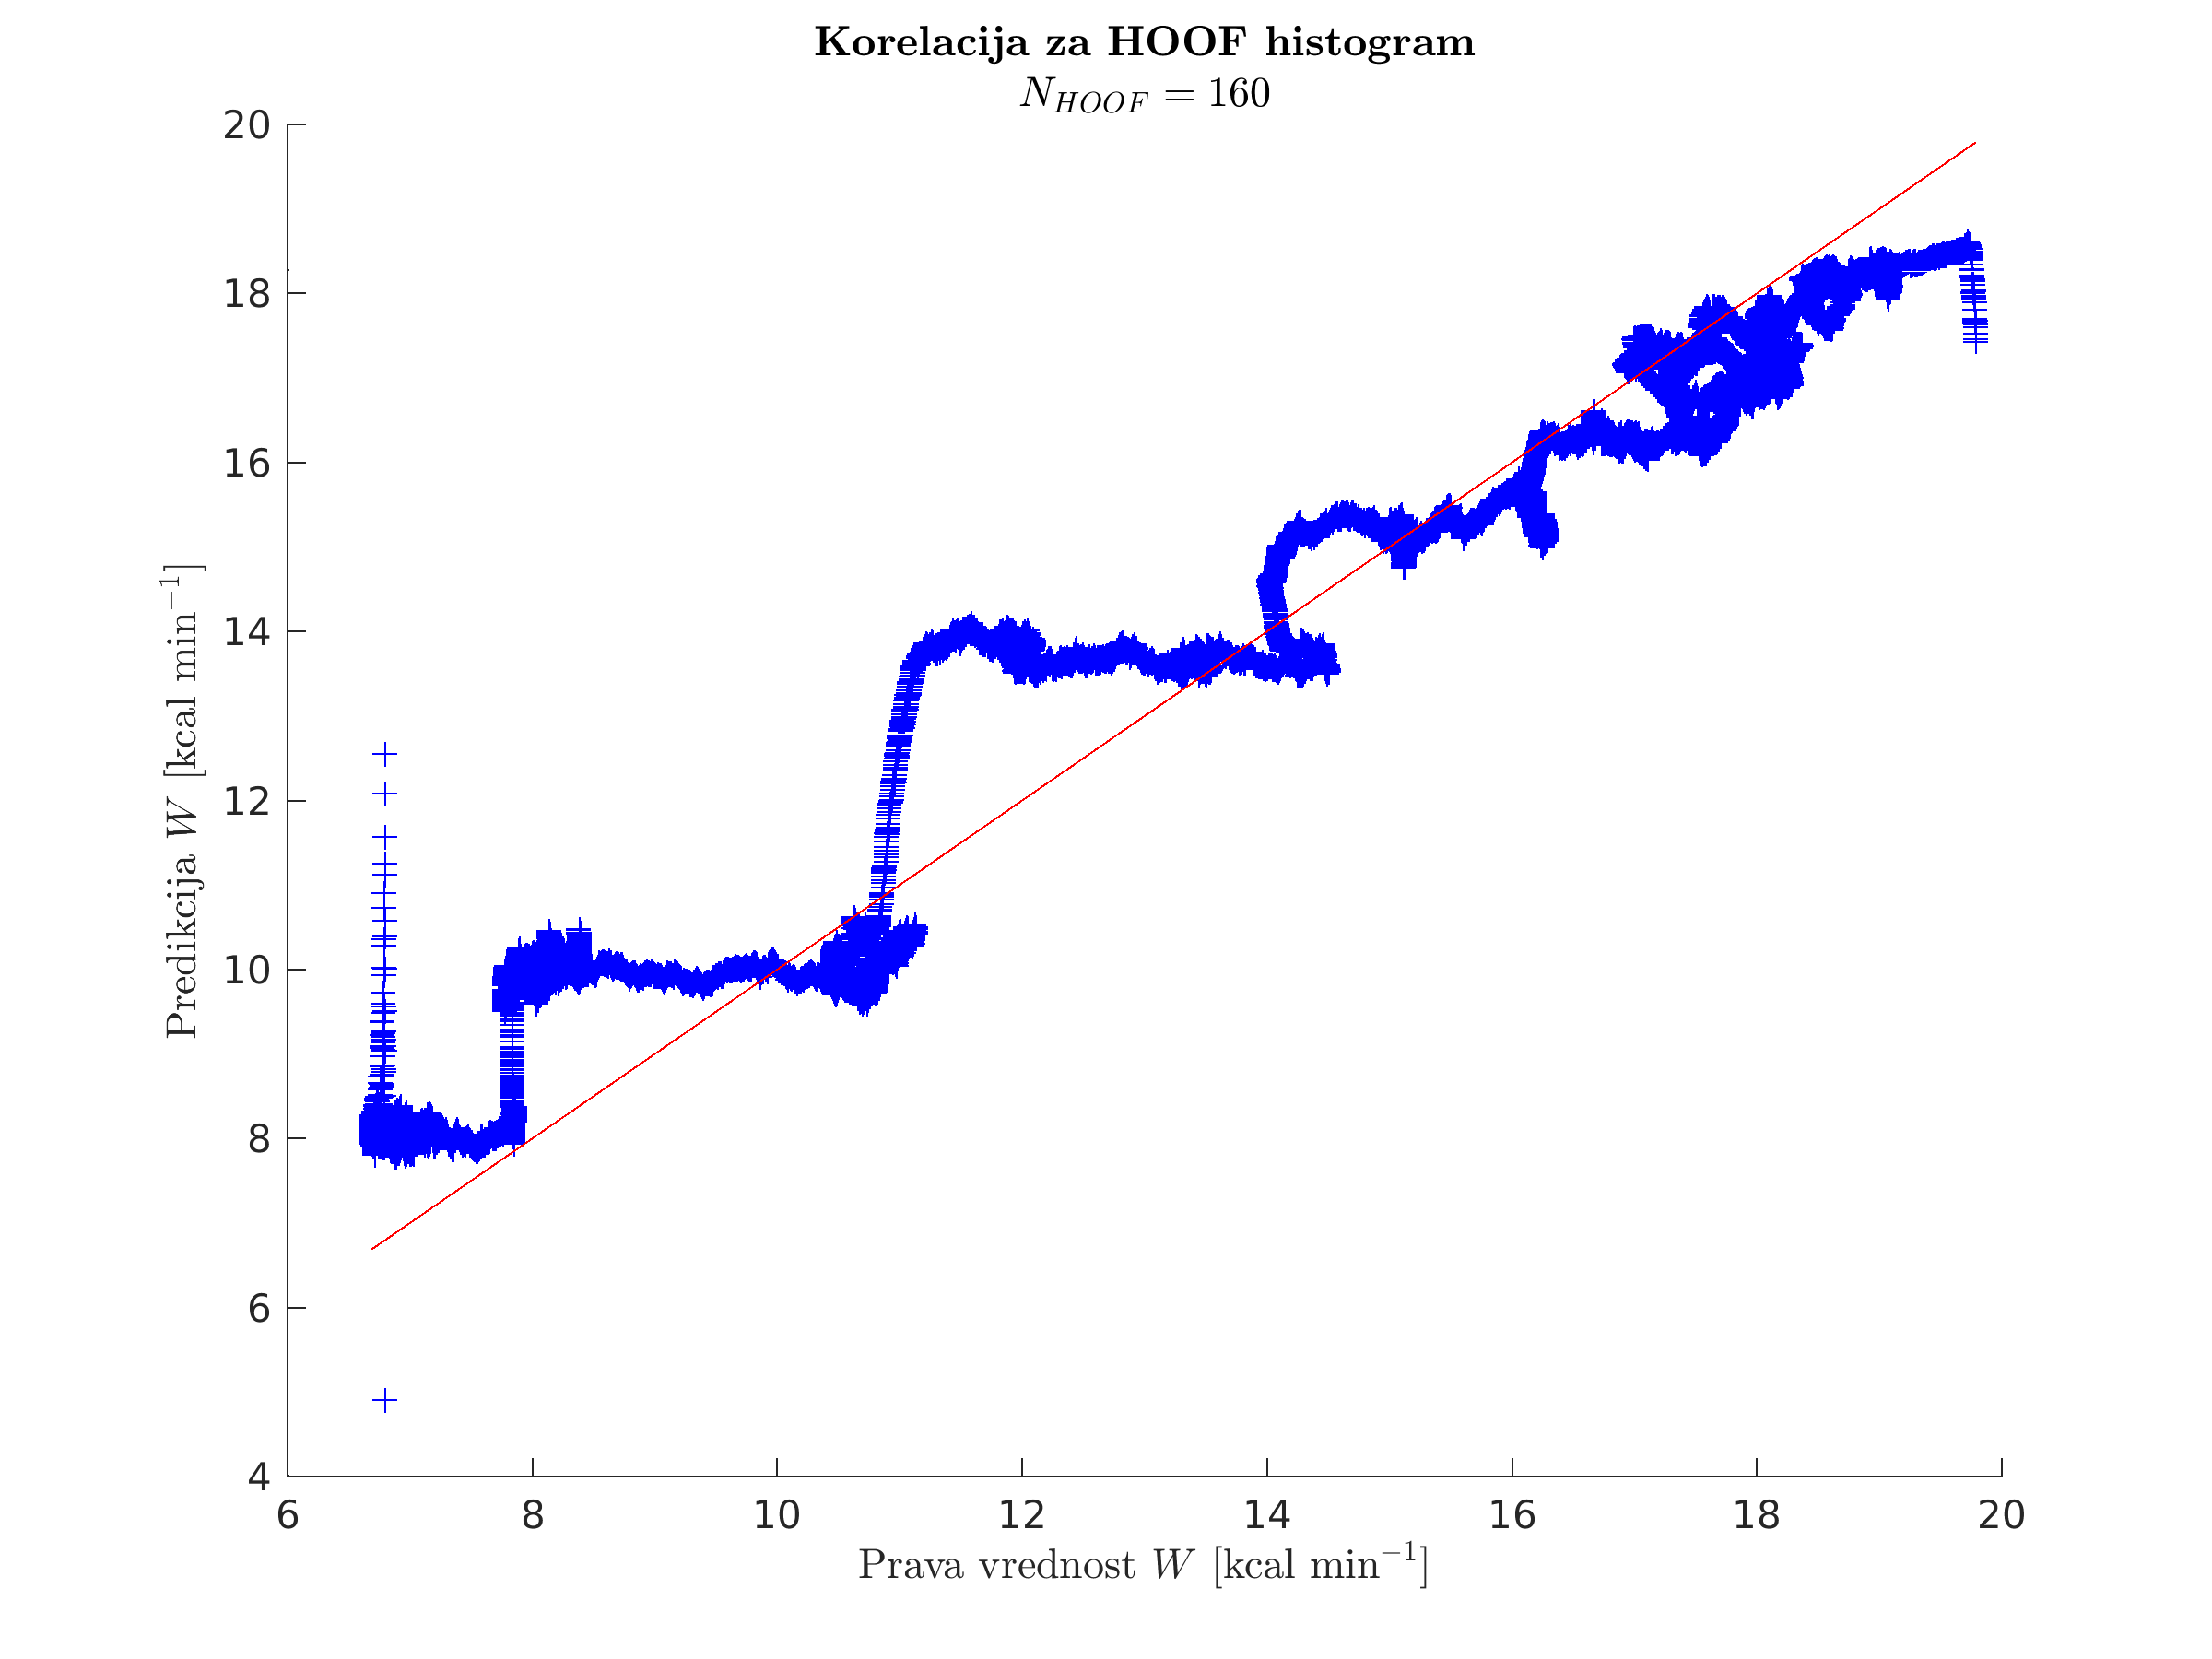
\includegraphics[width=\columnwidth]{./Slike/corr-hafa-160.png}
      \caption{Korelacija $N_{HAFA}=160$.}
      \label{fig:corr-hafa-160}
    \end{subfigure}
    \caption[Grafi korelacij modelov z različnim $N_{HAFA}$]{Grafi korelacij modelov z različnim številom stolpcev $N_{HAFA}$ HAFA deskriptorja. Rezultati so si zelo podobni.}
    \label{fig:corr-hafa}
\end{figure}





\subsubsection{Izbira deskriptorjev}

Chaudhry et al. \cite{chaudhry2009histograms} predlaga uporabo histogramov orientiranega optičnega toka (HOOF) za estimacijo gibanja. Vendar pa smo v preliminarnih terenskih testiranjih \cite{koporec2017observation} ugotovili, da njihova uporaba v realnih okoliščinah ni zadovoljiva. HOOF deskriptorju smo pripeli HAFA deskriptor in tako dobili razširjeni deskriptor HOOF-HAFA, ki v splošnem daje boljše rezultate, kot lahko vidimo v tabeli \ref{tab:izbira} in na primerjalnih slikah \ref{fig:izbira}.

Pri evaluaciji deskriptorjev HOOF in HOOF-HAFA smo uporabili učne vzorce hrbtne kamere terenskih testov. Evaluirali smo za podatke srčnega utripa $hr$. Srčni utrip smo za gradnjo modelov pretvorili v energijsko porabo $W$ po enačbi \eqref{eq:charlot}. Pridobljene značilke smo normirali na intervalu [0,1] in jih uporabili za učenje regresijskega modela z metodo podpornih vektorjev $\epsilon$-SVR in jedrom RBF. Za določitev optimalnih parametrov, ki so predstavljeni v tabeli \ref{tab:nhoof-param}, smo uporabili optimizacijsko metodo mrežnega iskanja \cite{hsu2003practical}. Rezultate smo filtrirali še s Gaussovim jedrom (predstavljen v \ref{sec:gaussov-filter}) velikosti $6$ in varianco $\sigma=16$. 

\begin{table}[htb]
	\centering
    \begin{tabular}{l S[table-format=2.3] S[table-format=1.3] S[table-format=1.3] S[table-format=1.3]}
    \toprule
    \textbf{Deskriptor} & \thead{$\mathbf{C}$} & \thead{$\mathbf{\gamma}$} & \thead{$\mathbf{\epsilon}$} & \thead{MSE} \\ 
    \midrule
    HOOF & 2.828 & 11.314 & 0.435 & 2.192 \\
    HOOF-HAFA & 5.657 & 2.828 & 0.154 & 1.781 \\
    \bottomrule
    \end{tabular}
    \caption[Optimalni parameteri RBF jedra modelov za izbiro deskriptorjev]{Optimalni parametri RBF jedra za modele z različnim deskriptorjem.}
    \label{tab:izbira-param}
\end{table}


\begin{table}[htb]
	\centering
    \begin{tabular}{l S[table-format=1.3] S[table-format=1.3] S[table-format=1.3] S[table-format=2.2]}
    \toprule
    \textbf{Deskriptor} & \thead{$\mathbf{r}$} & \thead{RAE} & \thead{RRSE} & \thead{nSV [\%]}\\
    \midrule%nSV
    HOOF & 0.992 & 0.336 & 0.317 & \boldentry{2.2}{82.34} \\%2187/2656
    \textbf{HOOF-HAFA} & \boldentry{1.3}{0.991} & \boldentry{1.3}{0.157} & \boldentry{1.3}{0.205} & 89.53 \\%2378
    \bottomrule
    \end{tabular}
    \caption[Rezultati evaluacije modelov z različnim deskriptorjem]{Rezultati evaluacije modelov z različnim deskriptorjem. Optimalni rezultati so odebeljeni. Vidimo lahko, da se bolje odnese razširjeni deskriptor HOOF-HAFA, čeprav model uporablja več podpornih vektorjev. }
    \label{tab:izbira}
\end{table}



\begin{figure}[htb]
	\centering
    \begin{subfigure}[t]{0.45\columnwidth}
      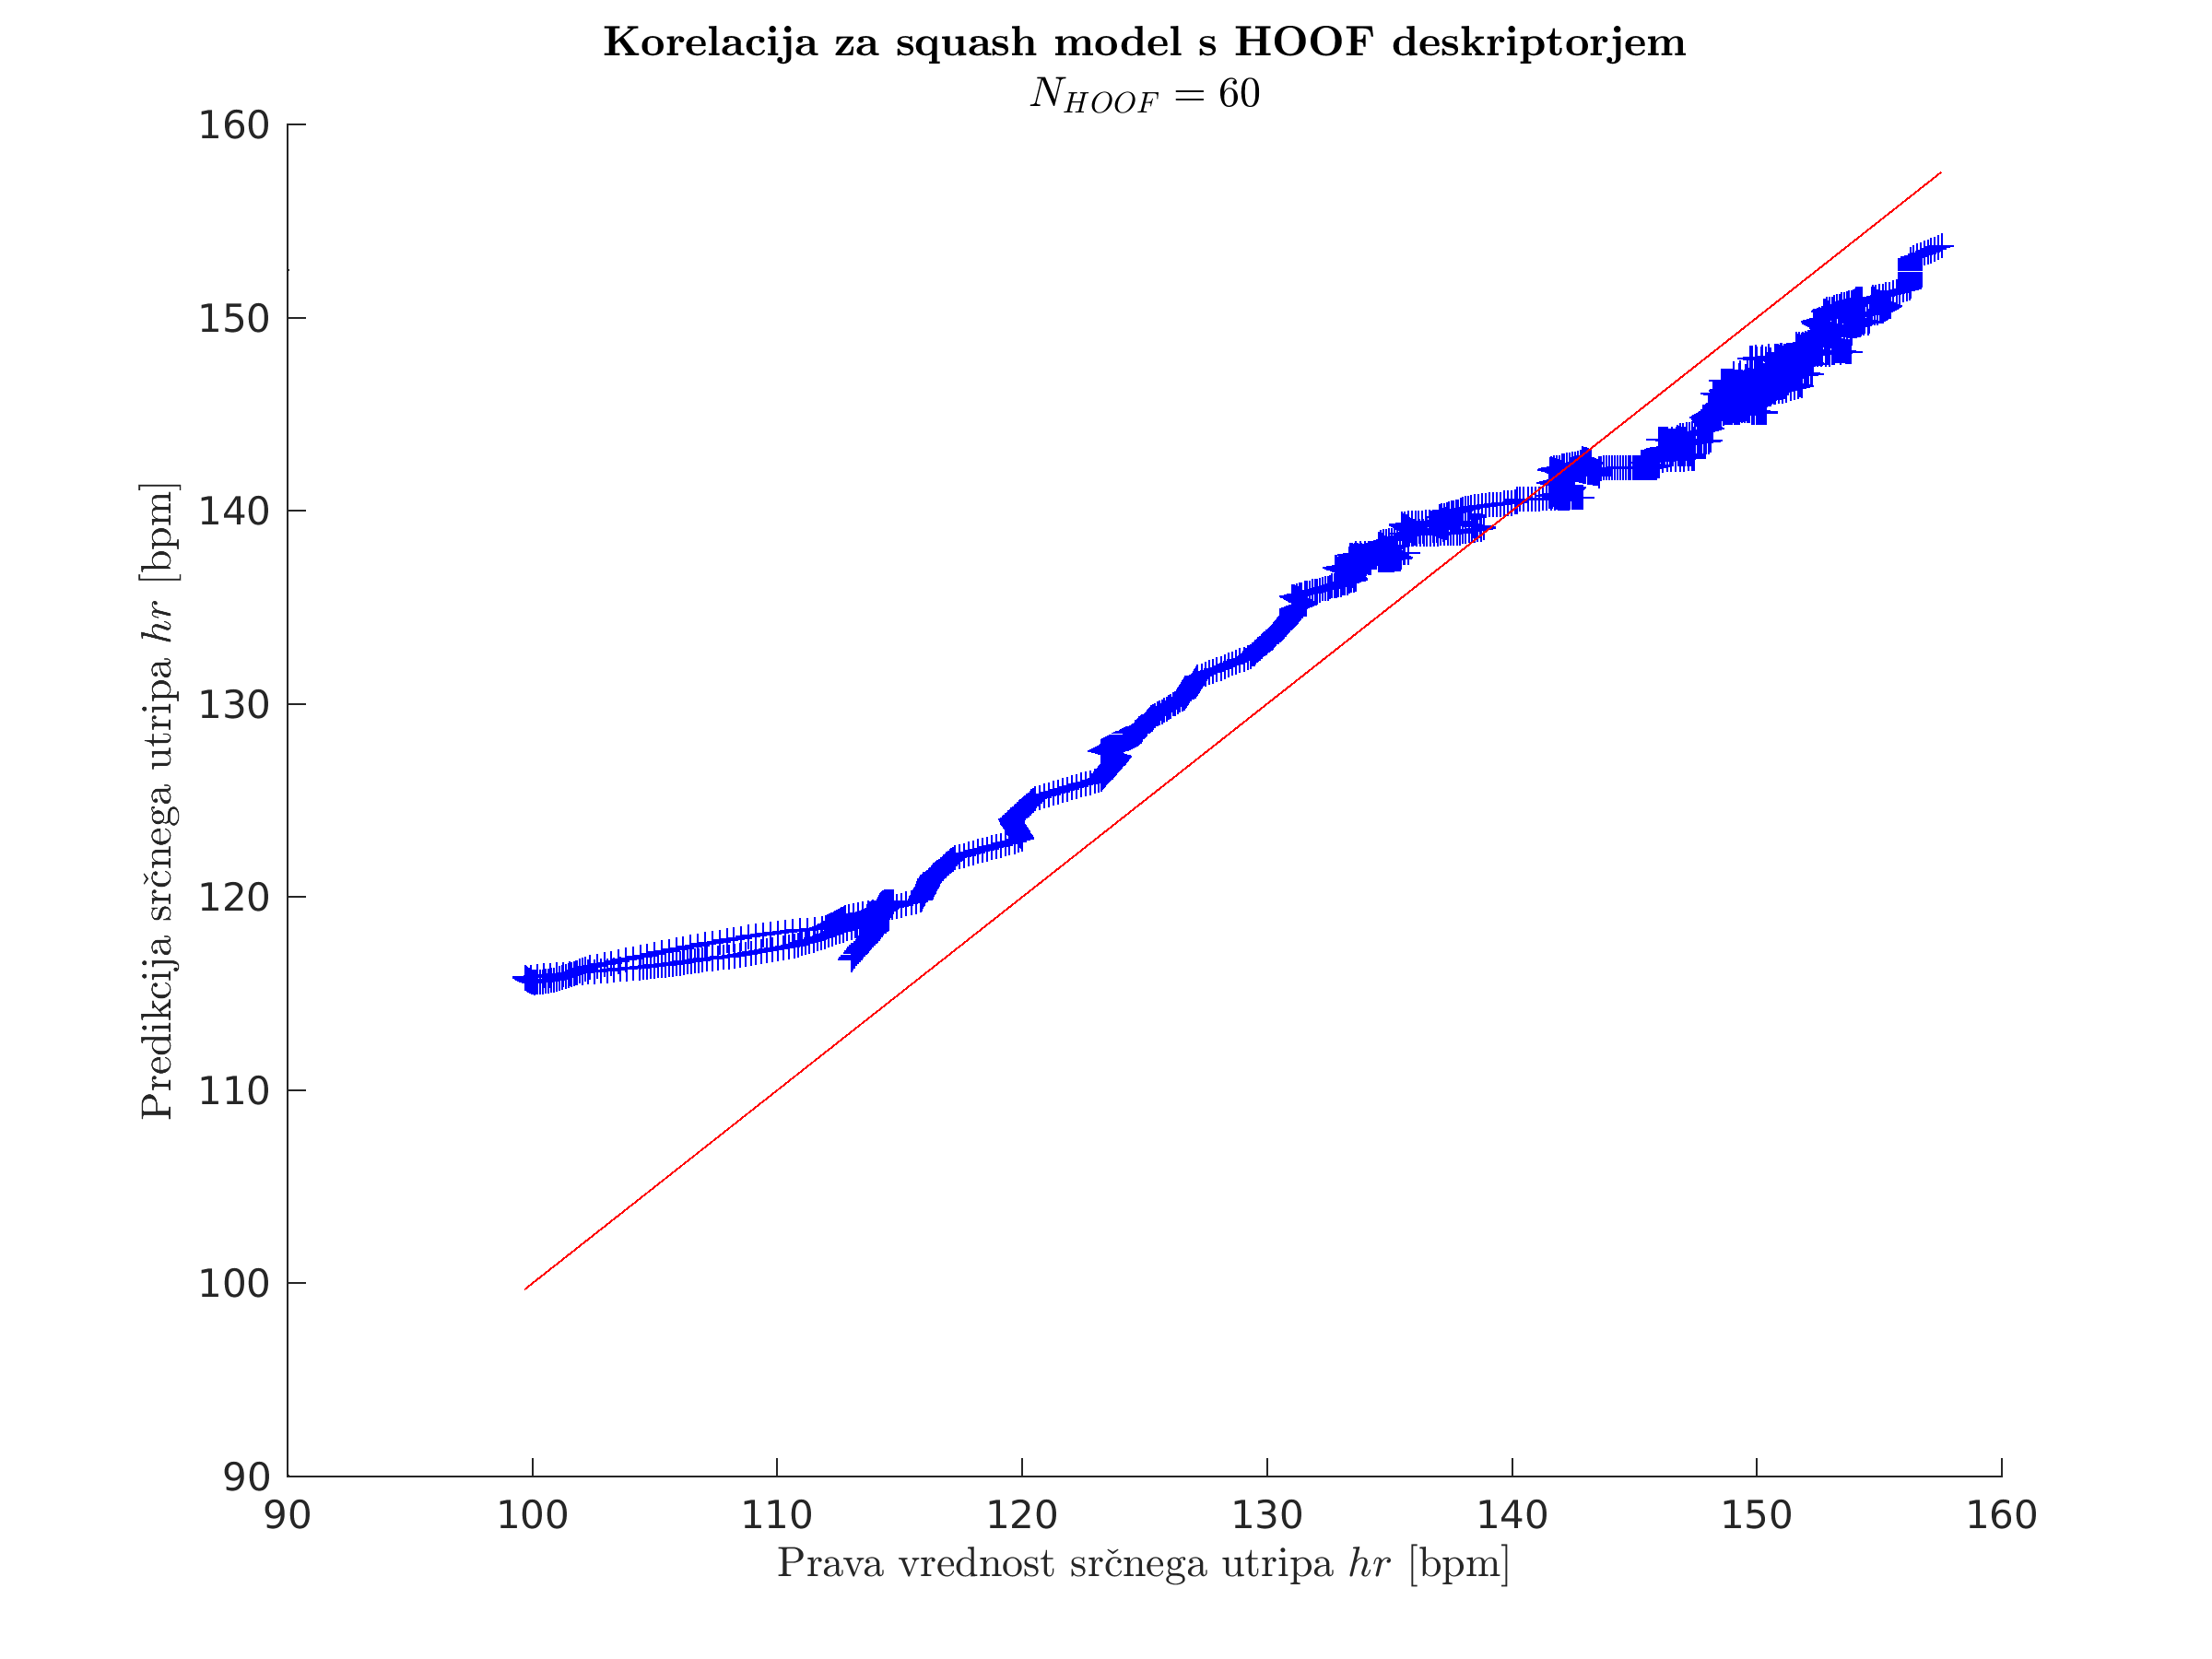
\includegraphics[width=\columnwidth]{./Slike/corr-hoof.png}
      \caption{Korelacija $N_{HOOF}=60$.}
      \label{fig:izbira-hoof}
    \end{subfigure}
    ~
    \begin{subfigure}[t]{0.45\columnwidth}
      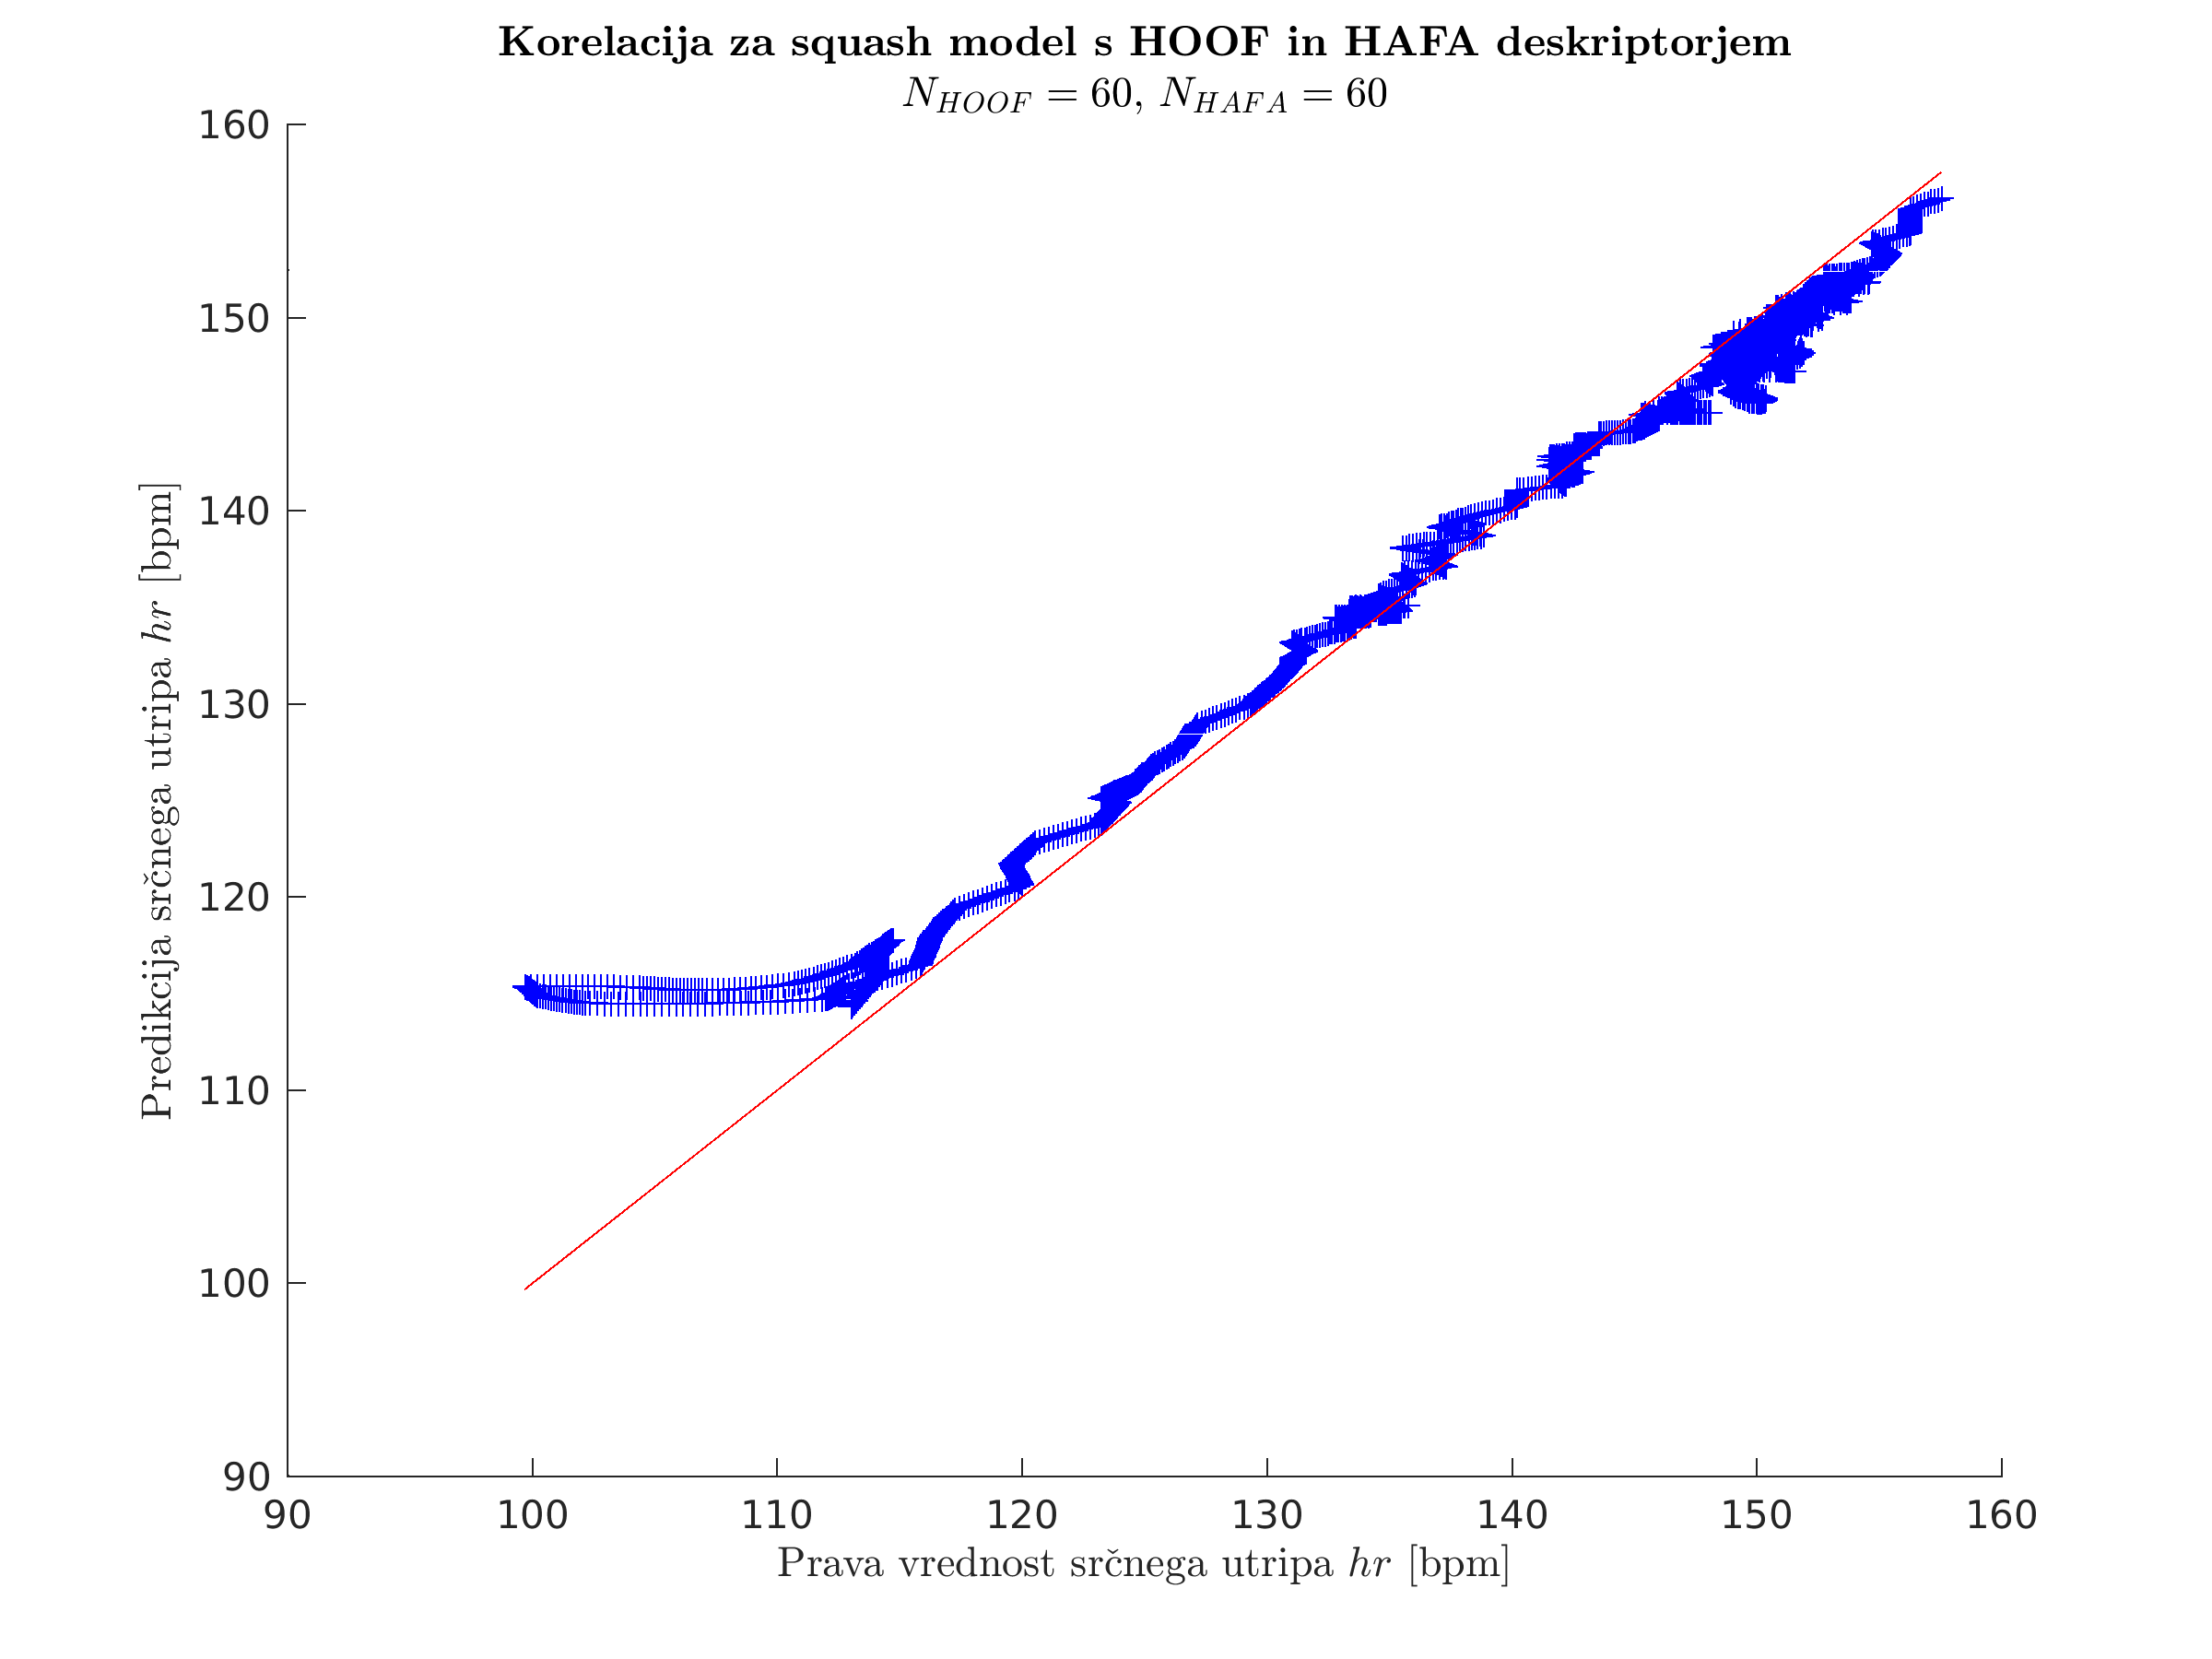
\includegraphics[width=\columnwidth]{./Slike/corr-hoof-hafa.png}
      \caption{Korelacija $N_{HOOF}=60$,\\$N_{HAFA}=60$.}
      \label{fig:izbira-hoofhafa}
    \end{subfigure}
    \caption[Primerjava modelov s HOOF in HOOF-HAFA deskriptorji]{Primerjava grafov korelacij modelov z različnimi deskriptorji. Model \subref{fig:izbira-hoof}) smo naučili s HOOF deskriptorjem. Model \subref{fig:izbira-hoofhafa}) smo naučili s HOOF in HAFA deskriptorjem. Posamezen vzorec je tako vseboval $120$ značilk. Pri primerjavi korelacije lahko opazimo vidno razliko. Model \subref{fig:izbira-hoofhafa}) dokazuje, da je razširjeni deskriptor boljši.}
    \label{fig:izbira}
\end{figure}













\subsection{Testiranje sledilnikov za optični tok}\label{sec:testiranje-sledilnikov-za-opticni-tok}
Sledilnike smo testirali na sekvencah slik \textit{handball1} in \textit{handball2} podatkovne baze VOT2016 \cite{kristan2016visual}. Sledila je še hitra vizualna ocena delovanja na kratkih izsekih video posnetka \cite{squashtv2014squash}.

Pri testiranju sekvenc slik podatkovne baze VOT2016 smo poenostavili rotirajoča referenčna področja detekcij na nerotirajoča področja. Pri tem smo za zgornji levi kot $T_0(x,y)$ in spodnji desni kot $T_1(x,y)$ uporabili enačbo \eqref{eq:vot-bb}, kjer so $\left( x_i, y_i\right), \forall i=1,\ldots,4$ ogljišča rotirajočega referenčnega področja. 

\begin{equation}
\begin{aligned}
	T_0(x,y) &= \left( \min_{i = 1,\ldots,4}\left\{x_i \right\}, 
    \min_{i=1,\ldots,4}\{y_i \} \right) \\
    T_1(x,y) &= \left( \max_{i = 1,\ldots,4}\left\{x_i \right\}, 
    \max_{i=1,\ldots,4}\{y_i \} \right)
\end{aligned}
\label{eq:vot-bb}
\end{equation}

Ker je za naš sledilnik najbolj pomembno zanesljivo delovanje, smo izbrali mero prekrivanja področja.


Video posnetek \cite{squashtv2014squash} smo za potrebe vizualne ocene delovanja na squash posnetkih razdelili na več kratkih izsekov. Pri tem smo uporabili le hrbtne posnetke mirujoče kamere. 

Rezultati testiranja so prikazani v tabeli \ref{tab:region-overlap}. Za izbrane sledilnike smo določili povprečje prekrivanja področja za posamezen posnetek. V tretjem stolpcu je predstavljeno povprečje prekrivanja glede na oba posnetka. Najboljši rezultati so odebeljeni. Po tabeli \ref{tab:region-overlap} se za posnetek \textit{handball1} najbolje izkaže CORR sledilnik. Za posnetek \textit{handball2} smo dobili najboljše rezultate pri sledilniku OPENCV-TLD. V povprečju se najbolje izkaže sledilnik CORR.




\begin{table}[htb]
	\centering
    \begin{tabular}{l S[table-format=1.3] S[table-format=1.3] S[table-format=1.3]}
    \toprule
    \textbf{Sledilnik} & \thead{$\mathbf{\Phi(\mathrm{handball1})}$} & \thead{$\mathbf{\Phi(\mathrm{handball2})}$} & \thead{$\mathbf{\overline{\Phi}}$}  \\
    \midrule%nSV
    NEBEHAY-TLD & 0.035 & 0.130 & 0.083 \\
    CCV-TLD & 0.117 & 0 & 0.117 \\
    OPENCV-TLD & 0.002 & \boldentry{1.3}{0.178} & 0.09 \\
    CORR & \boldentry{1.3}{0.214} & 0.160 & \boldentry{1.3}{0.187} \\
    \textbf{KCF} & {0.161} & {0.166} & {0.164} \\
    \bottomrule
    \end{tabular}
    \caption[Povprečje prekrivanja področja za posamezen sledilnik]{Povprečje prekrivanja področja za posamezen sledilnik in posnetek. V tretjem stolpcu je predstavljeno povprečje prekrivanja glede na oba posnetka. Najboljši rezultati so odebeljeni. Po tabeli \ref{tab:region-overlap} se za posnetek \textit{handball1} najbolje izkaže CORR sledilnik. Za posnetek \textit{handball2} smo dobili najboljše rezultate pri sledilniku OPENCV-TLD. V povprečju se najbolje izkaže sledilnik CORR.}
    \label{tab:region-overlap}
\end{table}


Na sliki \ref{fig:tracker-visual} lahko vidimo primer delovanja sledilnikov za oba posnetka. Referenčni igralec, ki mu morajo slediti ima rumeno majico. Za posnetek \textit{handball1} je predstavljena 15. slika, za posnetek \textit{handball2} pa 111. slika. Rezultati v tabeli \ref{tab:region-overlap} se skladajo z opažanji na sliki \ref{fig:tracker-visual}.

\begin{figure}[htb]
\centering

	\begin{subfigure}[t]{0.45\columnwidth}
      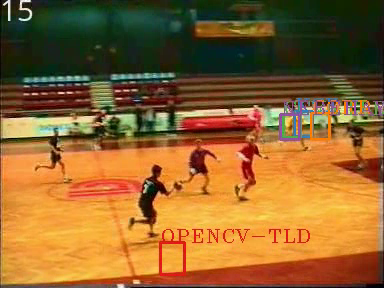
\includegraphics[width=\columnwidth]{./Slike/handball1-example.png}
      \caption{15. slika posnetka \textit{handball1}.}
      \label{fig:handball1}
    \end{subfigure}
    ~
    \begin{subfigure}[t]{0.45\columnwidth}
      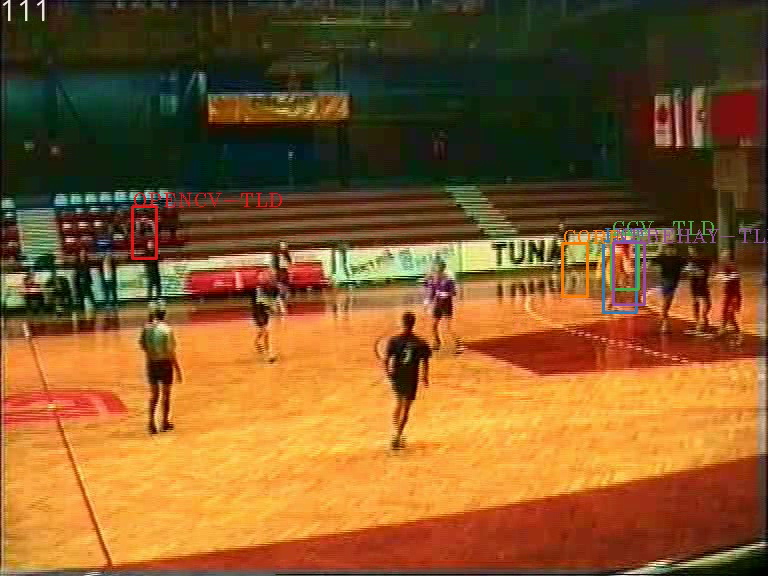
\includegraphics[width=\columnwidth]{./Slike/handball2-example.png}
      \caption{111. slika posnetka \textit{handball2}.}
      \label{fig:handball2}
    \end{subfigure}  
\caption[Primer delovanja sledilnikov za \textit{handball} posnetke]{Primer delovanja sledilnikov za \textit{handball} posnetke. Referenčni igralec, ki mu morajo slediti ima rumeno majico. }
\label{fig:tracker-visual}
\end{figure}




Čeprav smo z mero določili, da se je najbolje izkazal sledilnik CORR, se je pri hitri vizualni oceni sledenja na izsekih posnetka \cite{squashtv2014squash} izkazalo, da najbolje deluje sledilnik KCF. Primer boljšega delovanja KCF sledilnika je slika \ref{fig:squash-tracker-visual}, kjer sledimo modremu igralcu. Na isti sliki posnetka je KCF algoritem našel modrega igralca, medtem ko ga je CORR algoritem zamenjal z drugim igralcem. 



\begin{figure}[htb]
\centering

	\begin{subfigure}[t]{0.45\columnwidth}
      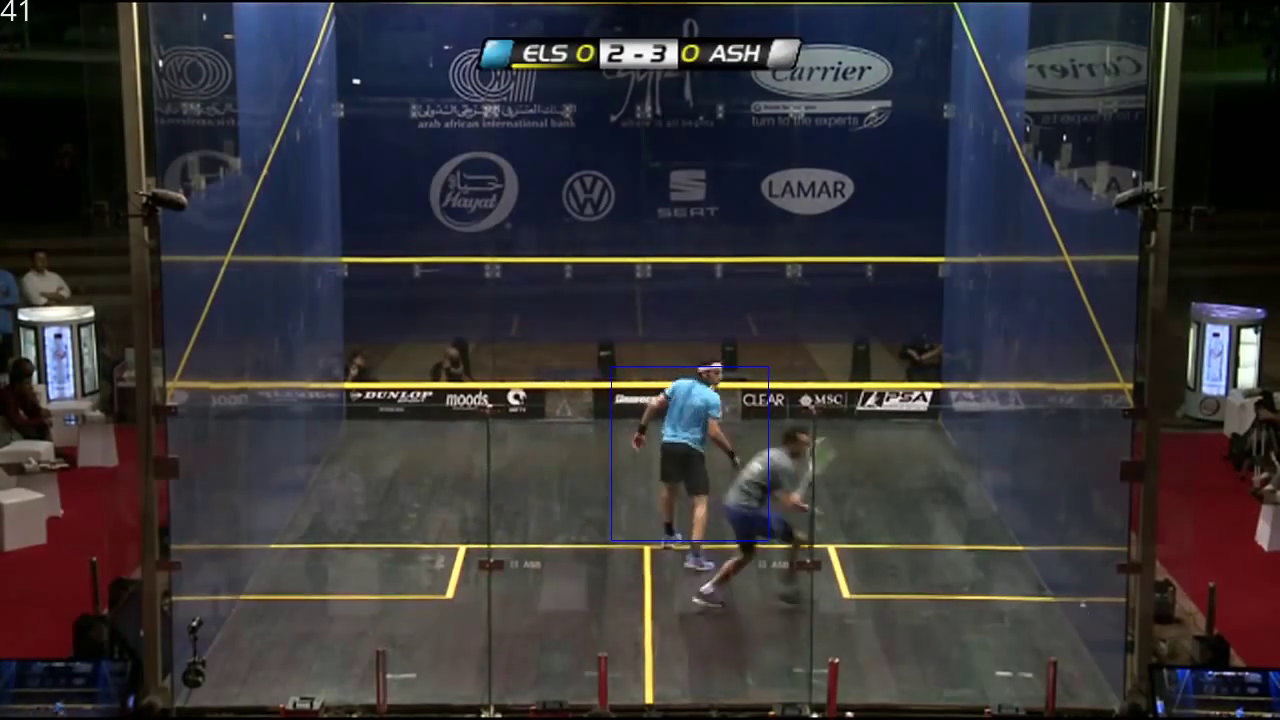
\includegraphics[width=\columnwidth]{./Slike/squash-1-kcf-example.png}
      \caption{41. slika posnetka \cite{squashtv2014squash} s KCF sledilnikom.}
      \label{fig:squash-1-kcf}
    \end{subfigure}
    ~
    \begin{subfigure}[t]{0.45\columnwidth}
      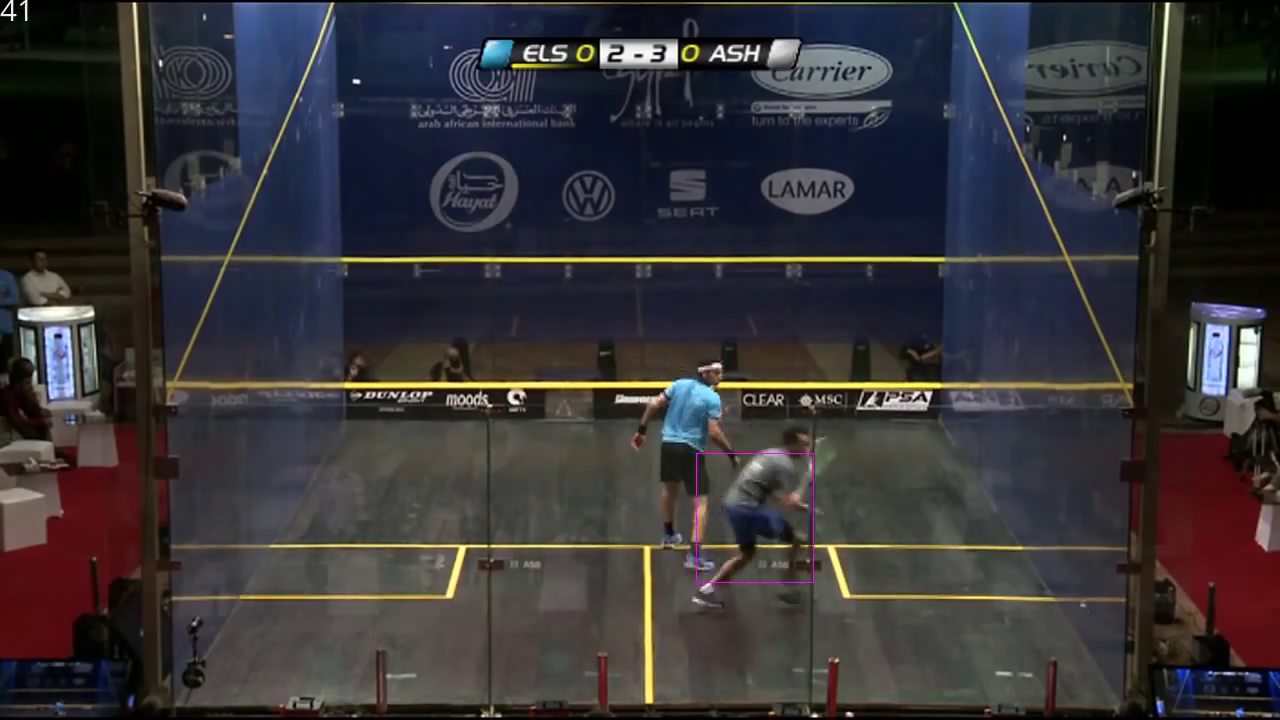
\includegraphics[width=\columnwidth]{./Slike/squash-1-corr-example.png}
      \caption{41. slika posnetka \cite{squashtv2014squash} s CORR sledilnikom.}
      \label{fig:squash-1-corr}
    \end{subfigure}  
\caption[Primer delovanja sledilnikov za squash posnetek]{Primer delovanja sledilnikov za squash posnetek. Gre za identični sliki posnetka, pri čemer smo na sliki \ref{fig:squash-1-kcf} uporabili KCF algoritem, na sliki \ref{fig:squash-1-corr} pa CORR algoritem. Sledilnika sta morala slediti igralcu z modro majico.}
\label{fig:squash-tracker-visual}
\end{figure}


Boljše delovanje KCF je razumljivo, saj prvi testi temeljijo na posnetkih rokometa, drugi pa na squashu, kjer gre za bistveno drugačno igro. Če pogledamo tabelo \ref{tab:region-overlap} ima KCF drugo najboljše povprečje, prav tako pa so si rezultati posameznih posnetkov zelo podobni. 









\subsection{Združevanje slik iz dveh Kinect kamer}\label{sec:zdruzevanje}
\subsubsection{Združevanje z značilkami}
Časovno sinhornizirana zaporedja slik smo nato poskušali združiti z metodo panoramskega šivanja slik z uporabo značilk, kot je opisano v delu \cite{brown2007automatic}. Tu smo namesto SIFT značilk uporabili SURF značilke.
Združevanje s značilkami se ni obneslo, zato smo to metodo opustili. Primer neuspelega poskusa je prikazan na sliki \ref{fig:zdruzevanje-znacilke}.

\begin{figure}[htb]
\centering
\begin{subfigure}[t]{0.45\columnwidth}
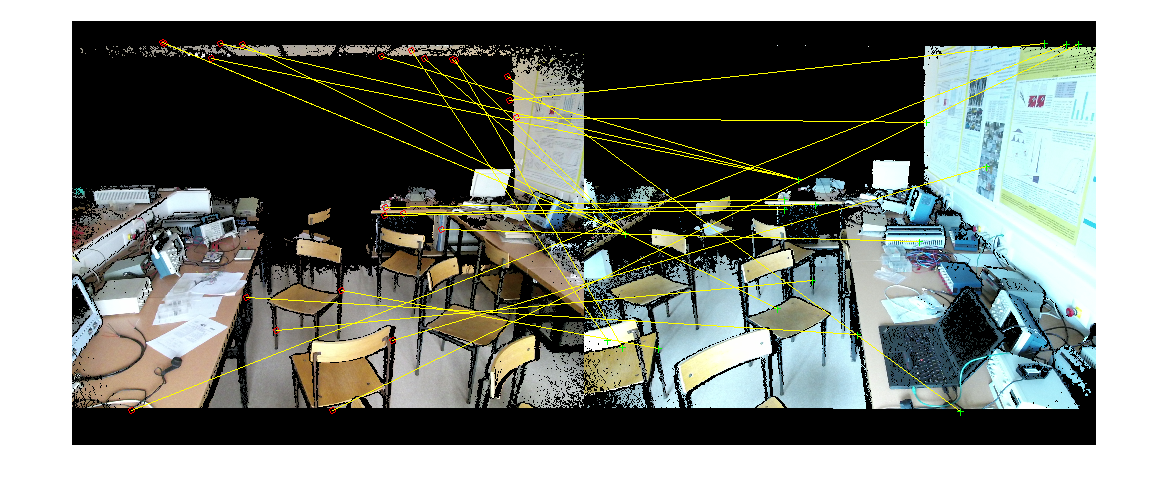
\includegraphics[width=\columnwidth]{./Slike/matched-features.png}
\caption{Ujemajoče SURF značilke}
\label{fig:zdruzevanje-surf}
\end{subfigure}
~
\begin{subfigure}[t]{0.45\columnwidth}
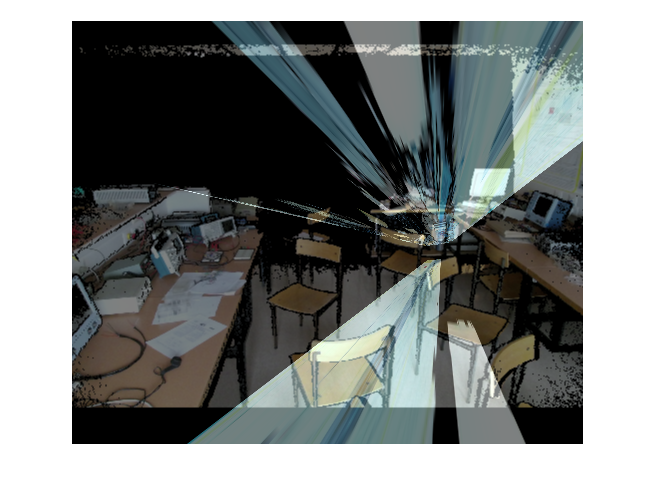
\includegraphics[width=\columnwidth]{./Slike/features-calibration-result.png}
\caption{Rezultat združevanja z značilkami}
\label{fig:zdruzevanje-result}
\end{subfigure}
\caption{Primer neuspelega poskusa združevanja slik iz dveh Kinect kamer s SURF značilkami.}
\label{fig:zdruzevanje-znacilke}
\end{figure}

\subsubsection{Združevanje s kontrolnimi točkami}
Zaporedja slik smo poskušali združiti z ročnim določevanjem kontrolnih točk. Rezultat je bil boljši od združevanja z značilkami, vendar še vedno slab, zato smo tudi to metodo opustili. Primer neuspelega poskusa je prikazan na sliki \ref{fig:zdruzevanje-cp}.

\begin{figure}[htb]
\centering
\begin{subfigure}[t]{0.45\columnwidth}
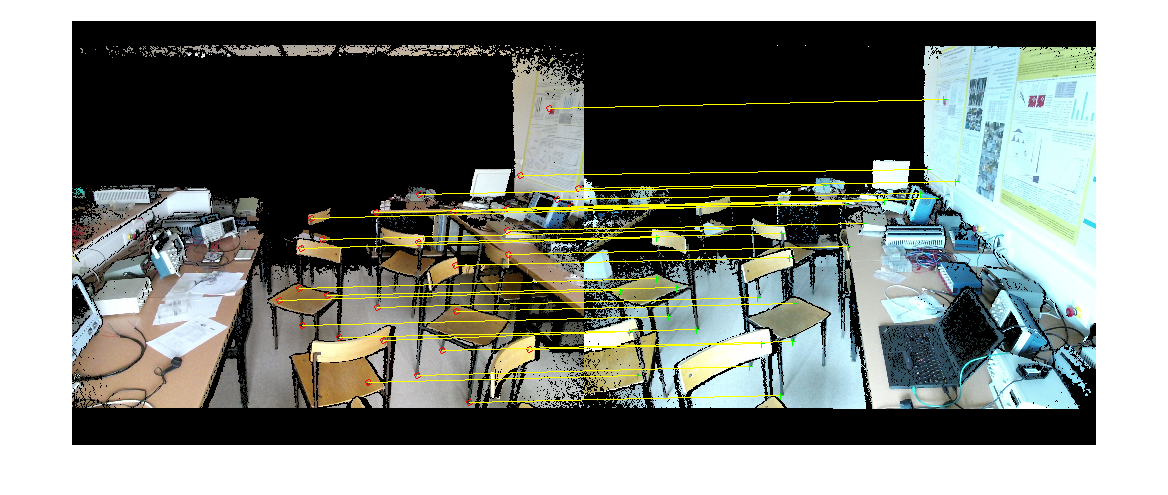
\includegraphics[width=\columnwidth]{./Slike/matched-points.png}
\caption{Ujemajoče kontrolne točke}
\label{fig:zdruzevanje-ujemajoce-cp}
\end{subfigure}
~
\begin{subfigure}[t]{0.45\columnwidth}
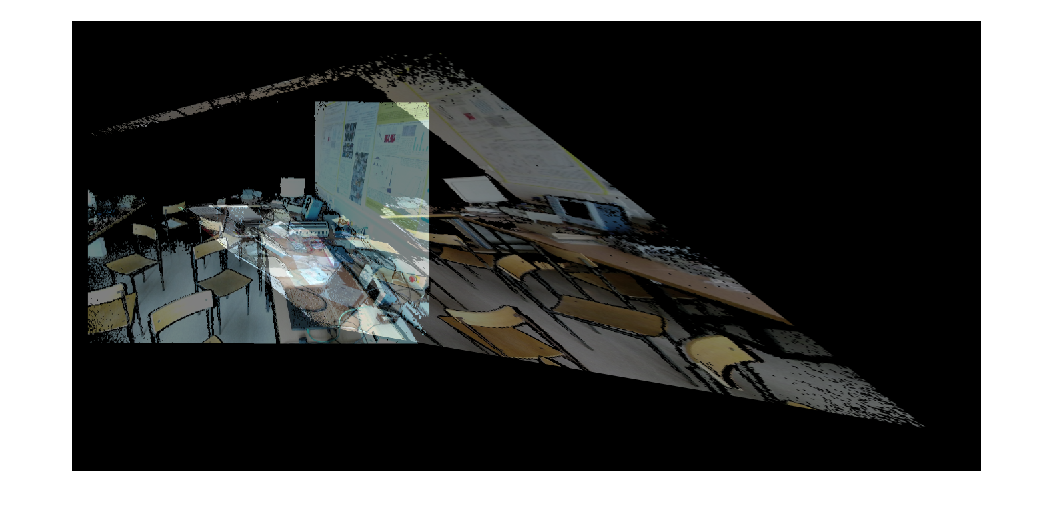
\includegraphics[width=\columnwidth]{./Slike/points-calibration-result.png}
\caption{Rezultat združevanja s kontrolnimi točkami}
\label{fig:zdruzevanje-result-cp}
\end{subfigure}
\caption{Primer neuspelega poskusa združevanja slik iz dveh Kinect kamer s kontolnimi točkami.}
\label{fig:zdruzevanje-cp}
\end{figure}


\subsubsection{Prilagojeno združevanje}
Zaradi nezadovoljivih rezultatov klasičnih metod združevanja stereo slik, smo razvili metodo, ki je prilagojena za Kinect kamere. Iz kamer smo pridobili intrinzične parametre infra-redečega (IR) senzora, in sicer: slikovni koordinati goriščne razdalje $f_u$ in $f_v$ ter slikovni koordinati optičnega središča slike (ang. principal point) $c_u$ in $c_v$. Intrinsične parametre smo uporabili za določitev intrizične matrike $\vec{M}_{int}$ po enačbi \eqref{eq:intrinsic}.


Ker pravih ekstrinsičnih parametrov kamer nismo poznali, smo jih le ocenili z metodo določevanja sečišča vidnih polj obeh kamer. Sečišče je prikazano kot rdeča linija na sliki \ref{fig:zdruzevanje}. S to metodo smo določili translacijski vektor $\vec{t} = \left [ t_x~ t_y~ t_z \right]^\top$ in rotacijsko matriko $\vec{R}$ iz Eulerjevih kotov.

S sledenjem igralca z DS-KCF algoritmom, smo s pomočjo projekcijske matrike \eqref{eq:projection-matrix} določili center tarče v metričnih enotah za vsako sliko zaporedja leve in desne kamere. Kadar slikovni element ni vseboval podatkov globine, smo za center tarče izbrali najbližji slikovni element z veljavno globino.

Prva slika združenega zaporedja je bila slika kamere, kjer se igralec prvič pojavi. Nadaljne slike smo izbirali med zaporedjema kamer glede na pozicijo centra tarče. Ko je šel center tarče skozi upragovljeno mejo, ki je na sliki \ref{fig:zdruzevanje} prikazana z modro linijo smo preklopili na drugo kamero. Razdalja med pragom in sečiščem je znašala \SI{200}{mm}.


\begin{figure}[htb]
\centering
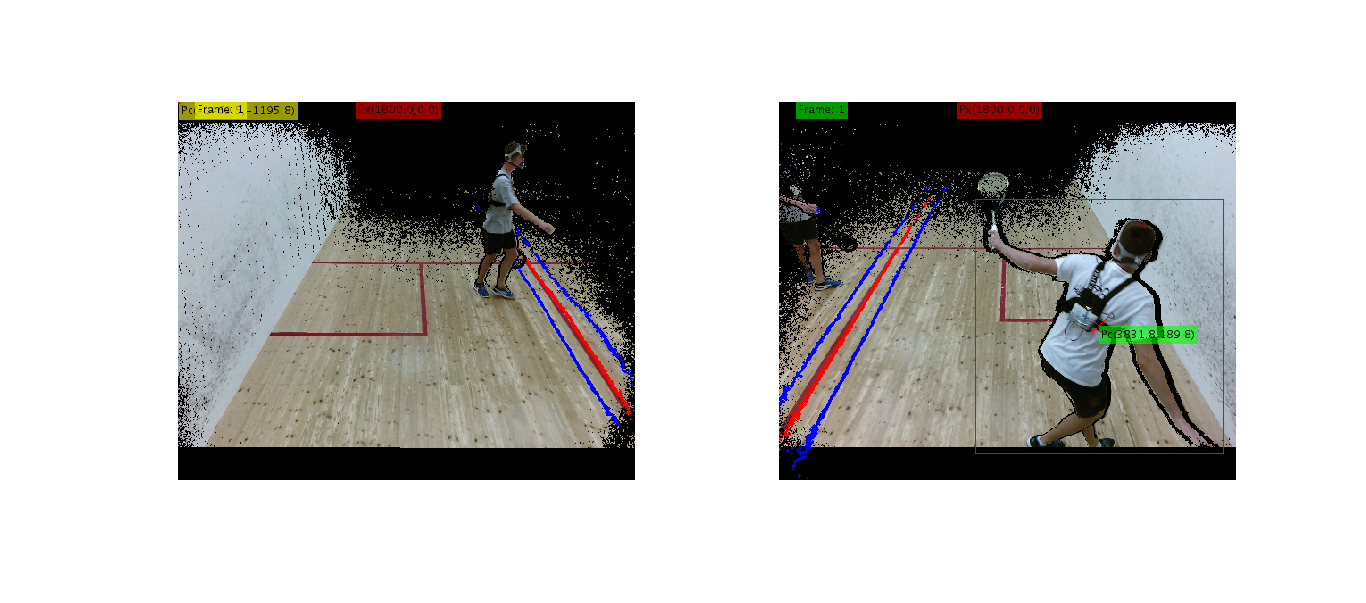
\includegraphics[width=\columnwidth]{./Slike/zdruzevanje-example.png}
\caption[Določevanje sečišča vidnih polj leve in desne Kinect kamere]{Določevanje sečišča vidnih polj leve in desne Kinect kamere. Na sliki sta prikazani prvi sliki zaporedja leve in desne Kinect kamere 1. seta 2. igre terenskega eksperimenta iz 2. faze. Označen je 4. igralec. Zelena barva koordiat središča tarče predstavlja izbrano kamero. Kamera z rumeno barvo ni izbrana. Sečišče je rdeča linija. Modri liniji sta pragova za preklop med kamerama. Ležita \SI{200}{mm} levo in desno od sečišča.}
\label{fig:zdruzevanje}
\end{figure}